
% Eric Valentino Master's Thesis

%%%%%%%%%%%%%%%%%%%% Imports %%%%%%%%%%%%%%%%%%%%

% \documentclass[hidelinks,12pt]{article}
\documentclass[12pt]{usfcoe}
\textheight  9.0in
% \usepackage[pdftex]{graphicx}

\usepackage{upgreek}
\usepackage{indentfirst}
\usepackage{xcolor}
\usepackage{csvsimple}
\usepackage{array}
\usepackage{epsfig}
\usepackage{wrapfig}
\usepackage{setspace}
\usepackage{epstopdf}
\usepackage{amsmath}
\usepackage{subfig}
\usepackage{float}
\usepackage[margin=1.0in]{geometry}
\usepackage[titletoc]{appendix}
\usepackage{chngcntr}
\usepackage{subcaption}
\usepackage{morefloats}
\usepackage{afterpage}
\usepackage{geometry}
\usepackage{setspace}
\usepackage{lipsum}
% From org mode
% \usepackage{graphicx}
\usepackage{grffile}
% \usepackage{longtable}
\usepackage{rotating}
\usepackage[normalem]{ulem}
\usepackage{textcomp}
\usepackage{amssymb}
% \usepackage{hyperref}
\usepackage{circuitikz}
\usepackage{amsmath}
\usepackage{cite}
% \usepackage[labelfont=it,textfont={bf,it}]{caption}
\graphicspath{ {./images/} }
% From https://tex.stackexchange.com/questions/254305/insert-pseudo-code-as-figure
\usepackage{algorithm}
\usepackage[noend]{algpseudocode}
% \usepackage{subfigure}
\usepackage{tocloft}
\usepackage[justification=centering]{caption}
\usepackage{titlesec}
% \captionsetup{justification=raggedright,singlelinecheck=false}
\captionsetup[table]{position=bottom}   % Make captions appear below table
%Taken from https://tex.stackexchange.com/questions/176157/table-caption-below-the-table

\doublespacing
\newpage
\makeatletter

%%%%%%%%%% USF COE Commands %%%%%%%%%%%%%%%

% Making all font 12pt as given in the formatting guide
% https://tex.stackexchange.com/questions/215920/force-font-size-for-entire-document
\renewcommand{\tiny}{\normalsize}
\renewcommand{\footnotesize}{\normalsize}
\renewcommand{\small}{\normalsize}
\renewcommand{\large}{\normalsize}
\renewcommand{\Large}{\normalsize}
\renewcommand{\LARGE}{\normalsize}
\renewcommand{\huge}{\normalsize}
\renewcommand{\Huge}{\normalsize}

\setlength{\abovedisplayskip}{3pt}
\setlength{\belowdisplayskip}{3pt}
% \setlength{\textfloatsep}{\baselineskip plus 0.2\baselineskip minus 0.5\baselineskip}




% This leaves a total of 2 inches to satisfy requirement for major headings
\newcommand{\usfpagebreak}{\pagebreak\vspace*{0.5in}} 

%  This command does a lot of hacky stuff. to put "chapter" before section number
\newcommand{\usfchapter}[1] 
{
    \pagebreak
    \vspace*{.72in}
    % \centering
    
	    % Increment the section number
        \addtocounter{section}{1} 
        % Make the section read "CHAPTER <section_num> <text>"
        \section*{\centering CHAPTER~\thesection: #1} 
        % Add the same to TOC 
        \addcontentsline{toc}{section}{CHAPTER~\thesection: #1} 
        % Reset the counters for sub sections. 
        \setcounter{subsection}{0} 
        \setcounter{subsubsection}{0}
	    % Note deeper depth counters will not be reset
% 	 \left
}

% Changing the space before and after display environments (tables, figures, etc.)
\g@addto@macro\normalsize{%
  \setlength\abovedisplayskip{10pt}
  \setlength\belowdisplayskip{10pt}
  \setlength\abovedisplayshortskip{10pt}
  \setlength\belowdisplayshortskip{10pt}
}

% Make the spacing between headings and text constant

% Telling latex to try to avoid orphans and widows
\widowpenalty10000
\clubpenalty10000

\makeatletter
\begin{document}

% Changing the space before and after display environments (tables, figures, etc.)
% \g@addto@macro\normalsize{%
%   \setlength\abovedisplayskip{10pt}
%   \setlength\belowdisplayskip{10pt}
%   \setlength\abovedisplayshortskip{10pt}
%   \setlength\belowdisplayshortskip{10pt}
% }
\newcommand{\usfcoespacing}{6pt}

\titlespacing{\section}{0pt}{0pt}{0pt}
\titlespacing{\subsection}{0pt}{0pt}{0pt}
\titlespacing{\subsubsection}{0pt}{0pt}{0pt}

\setlength\abovedisplayskip{0pt}
\setlength\belowdisplayskip{\usfcoespacing}
\setlength\abovedisplayshortskip{0pt}
\setlength\belowdisplayshortskip{\usfcoespacing}

% \setlength\parskip{\usfcoespacing}

%%%%%%%%%% Title Page %%%%%%%%%%%%%%%
\begin{titlepage}
	\fontsize{12}{14.4}
	\selectfont
	\singlespacing
	\begin{center}
		\vspace*{0.72in}
		The Design of Passive Networks with Full-Wave Component Models\\
		\vspace*{3\baselineskip}
		by\\
		\vspace*{3\baselineskip}
		Eric Valentino\\
		\vspace*{5\baselineskip}
		A thesis submitted in partial fulfillment\\ of the requirements for the degree of \\Master of Science in Electrical Engineering\\
		Department of Electrical Engineering\\
		College of Engineering\\
		University of South Florida\\
		\vspace*{3\baselineskip}
		Co-Major Professor: Gokhan Mumcu, Ph.D.\\
		Co-Major Professor: Lawrence Dunleavy, Ph.D.\\
		Isabella Bedford, M.S.E.E.\\
		\vspace*{2\baselineskip}
		Date of Approval:\\
		June 21, 2019\\
		\vspace*{3\baselineskip}
		Keywords:\\
		Full-Wave Modeling, Parasitic Effects, Component Interaction, Compact Passive Networks \\
		\vspace*{\baselineskip}
		Copyright~\copyright~2019, Eric Valentino
	\end{center}
\end{titlepage}
		
	
%%%%%%%%%% Dedication %%%%%%%%%%%%% 

\usfpagebreak
\thispagestyle{empty}
\begin{center}
\textbf{DEDICATION}\\
\normalfont 
To Mom and Dad. 
\end{center}
	
%%%%%%%%%% Acknowledgment %%%%%%%%%%%%%

\usfpagebreak
\thispagestyle{empty}
\pagestyle{empty}
\begin{center}
\textbf{ACKNOWLEDGMENTS}\\
\end{center}
	
The author would like to acknowledge Lawrence Dunleavy, Isabella Bedford, and Gokhan Mumcu for their continued assistance and mentorship.
Also worthy of recognition were those who assisted from Modelithics, Johanson, ANSYS, TDK and Rogers by supplying samples and providing support.
			
This research made use of scikit-rf, an open-source Python package for RF and Microwave applications.
%%%%%%%%%%%%%Table of Contents%%%%%%%%%%%%%%%%%%%
% YOu still have a 1.4.1 w/o a 1.4.2 
% Getting rid of table of contents dots for consistency between chapters and sections
\renewcommand{\cftdot}{}

\renewcommand{\cftlottitlefont}{\hspace*{\fill}\bfseries}
\renewcommand{\cftafterlottitle}{\hspace*{\fill}}
\renewcommand{\cftloftitlefont}{\hspace*{\fill}\bfseries}
\renewcommand{\cftafterloftitle}{\hspace*{\fill}}
\setlength\cftbeforefigskip{12pt}

\setlength{\belowcaptionskip}{0pt}


\usfpagebreak
\pagestyle{plain}
\pagenumbering{roman}
\setlength{\footskip}{.25in}

% Link to make sure headings are properly capitalized 
% https://capitalizemytitle.com/

% Making table of contents section entries not bold
\addtocontents{toc}{\string\renewcommand{\protect\cftsecpagefont}{\protect\normalfont}}
\addtocontents{toc}{\string\renewcommand{\protect\cftsecfont}{\protect\normalfont}}
\addtocontents{toc}{\string\renewcommand{\protect\cftsecleader}{\protect\normalfont\protect\cftdotfill{\protect\cftsecdotsep}}}

% Make the table of contents title, centered, bold, in normal font size
\renewcommand{\cfttoctitlefont}{\hspace*{\fill}\bfseries}
\renewcommand{\cftaftertoctitle}{\hspace*{\fill}}

% Make the indents 0.5" in each time
\cftsetindents{subsection}{0.5in}{2em}
\cftsetindents{subsubsection}{1in}{2.75em}

% Making the margins 0.5" away from the page numbers on the right
\cftsetrmarg{.95in}

\begin{spacing}{1}
    \tableofcontents
\end{spacing}

			
%%%%%%%%%%%%% List of Tables %%%%%%%%%%%%
\setlength{\cfttabindent}{0in}
\setlength{\cftfigindent}{0in}
\usfpagebreak
\begin{spacing}{1}
    % Putting "Table" before number
    \renewcommand{\cfttabpresnum}{Table }
    % pushing title over so it doesn't overlap with table number
    \setlength{\cfttabnumwidth}{0.7in}
    \setlength{\cftparskip}{\baselineskip}
    
    \addcontentsline{toc}{section}{LIST OF TABLES}
    \listoftables
\end{spacing}
\pagebreak

%%%%%%%%%%%% List of Figures %%%%%%%%%%%%

\usfpagebreak
\begin{spacing}{1}
    % Putting "Figure" before number
    \renewcommand{\cftfigpresnum}{Figure }
    % pushing title over so it doesn't overlap with figure number
    \setlength{\cftfignumwidth}{0.9in}
	\setlength{\parskip}{15pt}
    \addcontentsline{toc}{section}{LIST OF FIGURES}
    \listoffigures
\end{spacing}
\pagebreak

%%%%%%%%% Abstract %%%%%%%%%
\renewenvironment{abstract}
 {\small
  \begin{center}
  \bfseries \abstractname\vspace{-.5em}\vspace{0pt}
  \end{center}
  \list{}{%
    \setlength{\leftmargin}{0in}% <---------- CHANGE HERE
    \setlength{\rightmargin}{\leftmargin}%
  }%
  \item\relax}
 {\endlist}

\usfpagebreak
\begin{abstract}
    \doublespacing
    \addcontentsline{toc}{section}{ABSTRACT}
    
    \hspace{18pt} In this thesis, the design of passive networks with the aid of full-wave simulation software and geometry-based models of lumped elements is investigated. 
    This is done by examining the results of a number of simulation examples, as well as measured data from manufactured designs to compare against simulated equivalents. 
    One such example is a chip antenna evaluation board design, in which the PCB, antenna, matching components and connector are all modeled.
    When measured, the simulation agreed with the board's best matched frequency of 5.5 GHz to within 20 MHz.
    In another, a new antenna layout is generated from an existing evaluation design which, produced a match of about -15 dB at the design frequency with a similar bandwidth to that shown on the antenna datasheet on the first attempt at manufacture. 
    Additionally, a statistical experiment was conducted in order to provide insight into the phenomenon of coupling between lumped components, and to define clearly when it starts to become an important effect to consider. 
    For both chip capacitors and inductors, a behavioral model of how much crosstalk is present in a prospective circuit was developed which takes into account angle and distance between components, as well as case size. 
    Finally, a simple discrete gradient descent was implemented in a commercial full-wave simulation software in order to assist in the refinement of designs containing 3-D geometry-defined component models.
% Describe your best conclusions, information about what was achieved, and how 
	\pagebreak
\end{abstract}

%%%%%%%%%%%%%%%%%%%%%%%%%%%%%%%%%%%%%%%%%%%%%%%%%%%%%%%%%%%%%%%%%%%%%%%%%%%%%%%%
%                                   BODY
%%%%%%%%%%%%%%%%%%%%%%%%%%%%%%%%%%%%%%%%%%%%%%%%%%%%%%%%%%%%%%%%%%%%%%%%%%%%%%%%

% full-wave MODELS FOR PASSIVE COMPONENTS AND ANTENNAS  

\usfchapter{FULL-WAVE COMPONENT MODELS IN MICROWAVE DESIGN: PRECEDENT, JUSTIFICATION AND CONCEPTS}
\pagenumbering{arabic}
\counterwithin{figure}{section}

\subsection{Contributions of This Work}

    In this section, the scope of this document is introduced. 
    This thesis aims to answer three questions concerning full-wave component models: 
    \vspace{-\topsep}
    \begin{itemize}
        \setlength{\parskip}{0pt}
        \setlength{\itemsep}{0pt} 
        \item When they should be used?
        \item How they are used?
        \item What results can be achieved with them?
    \end{itemize}
    \vspace*{-9pt}
    Each of these questions is answered in the various points in the text indicated in the remainder of this section.
    
    \indent If the concern is whether they should be used for a design in which lumped elements are closely spaced, then, depending on the substrate used, the question may be made clear by the behavioral model of coupling based on properties of the circuit developed in Section 2.4.1.
    Alternatively, if the concern is that the components are in too unusual of a configuration to be appropriately modeled by circuit models or S-parameters taken on microstrip, then it is likely a good application for full-wave component models.
    Specifics concerning this idea are discussed in more detail throughout the thesis.

    \indent Secondly, their use is demonstrated in the descriptions of how the two antenna design simulations of Chapter 3 are constructed. 
    In addition to these, a discrete gradient descent script has been implemented in the full-wave solver used which allows entire geometries to be swapped out such that the design can be optimized without the conscious attention of the designer.
    Given the long simulation times inherent to simulation, this can transform a full-wave design representation from a circuit simulation validation into it's own design tool.
    Though the use of this simulation is not explained in this thesis, the algorithm is important to use of full-wave models and has it's logic and implementation described in Section 1.5.2.
    
    \indent Lastly, the accuracy of the models and what kind of design results can be achieved with them is demonstrated by the measured impedance and radiation data in comparison with simulated responses.
    These comparisons can be seen at the end of each of the antenna design example sections of Chapter 3, and at the end of Chapter 2.
    
    Before moving on to discuss related work, it should be pointed out that while most of the results and conclusions apply generally to other simulators, in this work, demonstrations are performed using the commercially available High Frequency Structure Simulator (HFSS)  full-wave electromagnetic tool available from ANSYS. 
    HFSS uses a well-established numerical approach to solving Maxwell's equations known at the Finite Element Method (FEM).  
    Designs and components to be modeled by FEM must be defined by their material and three-dimensional geometry details (the representation of the latter is hereafter referred to as ``3-D'' or ``full-wave'' models). 
    Packaged alongside HFSS is also a circuit simulator that can simulate models defined by lumped equivalent circuit elements or S-parameter files.  
    The circuit simulator is also integrated with HFSS in such a way which allows an S-parameter representation of a solved HFSS design which may be connected to other components in the circuit schematic. 
    Simulating in this fashion will be referred to as ``co-simulation'', and is used often in this thesis.

\subsection{Related Work}
		
    \indent As RF and microwave designs move to higher frequencies and designs become smaller, designers are increasingly moving to full-wave simulators to gain confidence in their final designs. 
    Both planar and full-wave electromagnetic simulations are popular among those designing distributed microwave networks, but as of today, full-wave simulation for lumped passive components is yet to be widely adopted.
    Full-wave simulations have been used historically to inform equivalent circuit models as in \cite{LumpedElementHemtParasitics}, but the roadblocks of computing power and component vendors' need to protect intellectual property have, to date, kept full-wave analyses from being widely adopted for design work  for circuits involving lumped components. 
  
    % Computing Power

    However, these roadblocks have been starting to cede.
    In the case of computing power, research is being done into the parallelization (and subsequent speeding) of numerical electromagnetics solvers.
    In \cite{GPUOptimization} the speeding of an algorithm to formulate a integral-form electromagnetics problem into the standard matrix inversion problem is shown. 
    Over the two case studies given, a combined CPU and GPU approach to the problem yielded a speedup of 54x for some parts of the matrix construction. Also, in the specific field of using the finite-element method for electromagnetics, portions of the process of formulating and solving the problem have been sped up multiple times over, as is seen in \cite{GPU1}, \cite{GPU2}, and \cite{GPU3}.
    % Using Full-Wave Analysis to Extract Circuit Models

    For the aforementioned reasons, full-wave analysis has often been used as a reference to extract circuit models from for use in circuit simulators by designers, but in many cases, it can be more efficient to simply use the response of the full-wave simulations themselves. 
    Reference \cite{HEMTDistributedCircuitExtraction} shows the extraction of a transmission line based representation of HEMT parasitics from an HFSS representation of the structure to be measured. 
    It is novel in that it uses a more physical representation of the FET structure, then it may have been quicker and more accurate. 
    As detailed in the paper, the fitting process a full-wave simulation of increasing complexity must be run 6 times to extract the model for one geometry, and the scalability of the model to new geometries was not investigated, for the purposes of predicting the behavior of the parasitic model it seems that one full-wave analysis would be more efficient.
    However, this is not to say that the creation of the circuit model in \cite{HEMTDistributedCircuitExtraction} was not a worthy endeavor, as equivalent circuit models such as these provide a good conceptual understanding of how a part of a design is behaving electrically.
    % \cite{LumpedElementHemtParasitics}

    The use of full-wave electromagnetic modeling for design is also expanding outside it's traditional application of passives and antennas for RF and microwave applications.
    The paper referenced by \cite{FullWaveHemt} shows an interesting solution to the problem of modeling the channel of a HEMT, using a ``hydrodynamic'' set of constraints on the charge carriers in conjunction with a standard electromagnetic simulation.
    Though in this work the results are only validated against analytical expressions for the propagation constant of the channel, this approach could feasibly predict the response of a manufactured transistor for an arbitrary geometry and process.
    Outside the field of RF, those working on the frontier of power systems, as in \cite{FullWaveHighFrequencyLModeling} can also utilize full-wave analysis of components to gauge EMI and to get the most accurate picture of their device's performance.
    %   TODO look into FASTHENRY inductance extraction? 
        % M. Kamon, M.J. Tsuk, and J.K. White, “FASTHENRY: A Multiple-
        % Accelerated 3-D Inductance Extraction Program,” IEEE Trans.
        % Microwave Theory and Techniques, pp. 1750-1758, 1994.
    % Using Full-Wave Analysis just to model stuff

    

    \subsection{Background on Commercial Technology Used in this Thesis}

    Besides the obstacle of computing power, component manufacturers' (or ``vendors'') interest in keeping their intellectual property safe prohibits them from distributing the geometry and material composition of their components. 
    ANSYS HFSS, the full-wave electromagnetics simulator discussed earlier, has been making progress in this area.
    %https://www.ansys.com/-/media/ansys/corporate/resourcelibrary/techbrief/ab-ansys-hfss-3d-data-sheet.pdf
    % TODO take specific brand names out of this
    Recently, HFSS has introduced a system which allows designs to be modularized into encrypted sub-designs, encapsulating their geometry and material information, meshing operations, and variables. 
    This allows 3-D components to simulate accurately while hiding their internal geometry and material properties from the user.  
    With this development, manufacturers and modeling services now have a viable way to distribute full-wave component models without revealing the intellectual property of the manufacturers.  
    
    Given this, some companies % including  Johanson Technology, Inc. and Modelithics, Inc. 
    have  released full-wave encrypted 3-D models of commercially available electrical components intended for direct use by the designer.  
    With versions of ANSYS HFSS 18.3 or later, a component palette of various Johanson chip antennas is included, any of which which the designer can drop into their design in order to evaluate the gain, efficiency and match of an antenna design entirely with simulation.  
    \subsubsection{Scalable Equivalent Circuit Models}
    Also used in this text is the Modelithics CLR Library of substrate-scalable equivalent circuit models for many common capacitors, inductors, and resistors, which will be referred to as ``Modelithics' Global Microwave  Models'', or just ``Global Models''. Modelithics is a company which specializes in providing circuit models of many types of components commonly used in microwave circuit design.
    The global models in question are validated against measured data over different substrate heights and part values, and in addition, feature solder pad de-embedding, pad scaling, and support for statistical simulations.
    
    \subsubsection{Full-Wave Component Models}
    
    Beginning in 2018, Modelithics began adding a 3-D component library of various passive components to add  to it's ANSYS EDT compatible component equivalent circuit models. These 3-D models allow the designer to predict the effects of unusual configurations or interaction between components on any microwave design, as demonstrated in \cite{mdlx_3d_models} and \cite{HFSS_3d_components}. 
    These types of models will be used throughout this text and will be referred to as ``3-D Models'' or ``Full-Wave Models''.
    
    Though the effects of interactions between components and each other or their environment can be a second thought to many microwave designers, they can can have a very significant effect on the response of compact filters, matching networks and other designs involving passives.  
    Below, Figure 7 and 8 of \cite{mdlx_3d_models} are shown, in which the measured response of 3 closely-spaced 1.6nH CoilCraft 0603CS inductors is compared both to a circuit simulation using Modelithics' circuit model of the part, as well as the newly made HFSS model of the same.
    
    \begin{figure}[H]
        \begin{center}
        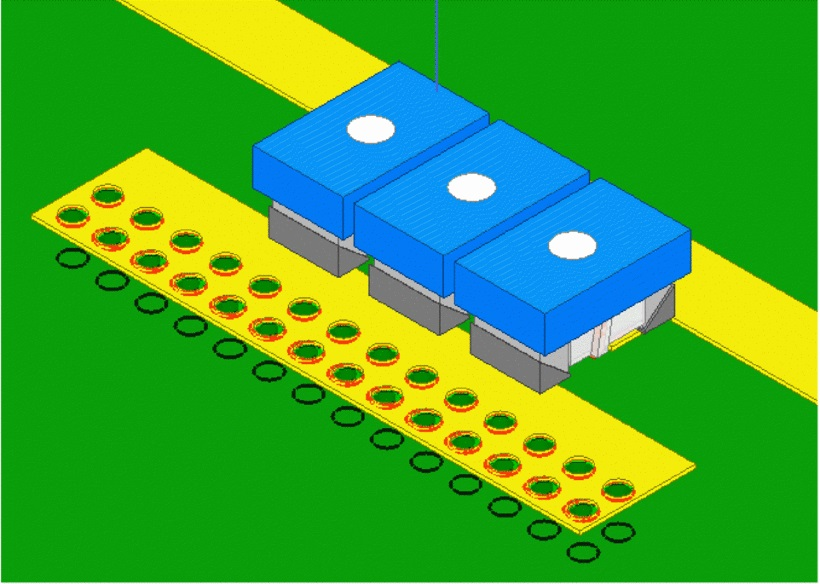
\includegraphics[width=3.5in]{images/mdlx3d_comps_paper_fig_7.jpg}
        \caption{Figure 7 of \cite{mdlx_3d_models}: Coupling example with three shunt 1.6nH Coilcraft 0603CS inductors placed with various spacings on a 50 $\Omega$ transmission line on 16mil Rogers 4003C \textcopyright \,  IEEE 2018.} 
        \label{fig:mdlx3d_comps_paper_fig_7}
        \end{center}
    \end{figure}


    \begin{figure}[H]
        \begin{center}
        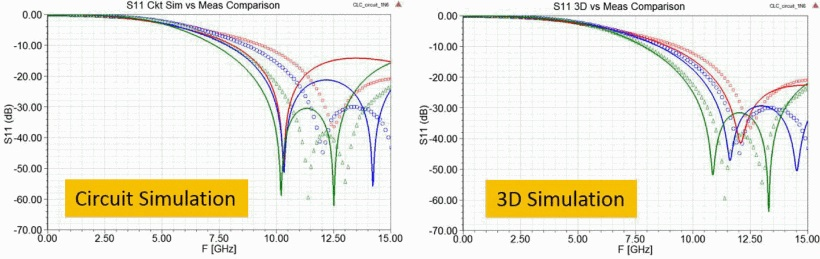
\includegraphics[width=\textwidth]{images/mdlx_3d_comps_paper_fig_8.jpg}   
        \caption{Figure 8 of \cite{mdlx_3d_models}: Legend for inductor spacings: Red - 10 mils, blue - 42 mils, green - 74 mils \textcopyright \, IEEE 2018.}
        \label{fig:mdlx3d_comps_paper_fig_8}
        \end{center}
    \end{figure}

    At the closest spacing, the circuit model predicts the self resonance of the part to be about 2 GHz less than it actually occurs, whereas the 3-D component model is less than 500 MHz off.  
    The ability to trust your models in such extreme configurations as these allows the microwave designer to attain the maximum performance of their parts, and precludes costly and time consuming revisions.  
    
    Though there are many cases where properly made circuit models are more appropriate and efficient to use than 3-D models \cite{ltcc_filter}, there are other cases in high-performance designs where the accuracy provided greatly helps for final pre-manufacturing validations and design optimization as well.  
    As alluded to in the introduction, the appropriate cases fall roughly into two categories: designs in which components are very closely spaced together, and designs in which components are in non-traditional configurations. 

    \subsubsection{Cosimulation with Brick Models}
    \label{differential_port_explanation}
    Lastly, a relatively new type of model, a hybrid between a full-wave and a circuit model, is the ``brick'' component model.
    A ``brick'' model uses full-wave analysis to model the terminations of the device, and uses an equivalent circuit to model the inside of the device.
    The idea of simulating part of a component in a full-wave simulator and the rest in a circuit simulator has been seen at least as far back as 2012, when \cite{brick_diode} was published, which achieved good measured to modeled agreement by approximating a  diode at a specific bias as a series RC circuit and introducing a boundary with the same R and C value in the full-wave simulator. 
    In ANSYS EDT, where this approach has been implemented, the circuit simulation is the top-level simulation, and a block representing the S-parameters of the full-wave simulation is placed in the circuit simulator with it's ports broken out.
    In order to avoid re-counting the effects of the terminations, there is a mode in the circuit model which removes parasitics corresponding to the package of the device, which is called the ``Simplified Parasitics Mode''. 
    The full-wave portion of the brick model can be seen in Figure \ref{fig:brick_model} .
    As shown, there is only one port, even though the circuit simulator representation of the inside of the device (the model in ``Simplified Parasitics Mode'') has two ports.
    %Future: Make graphic with two ways of co-simulating with circuit simulator, with 4 pictures, one with two HFSS ports from end of microstrip to ground, one with one differential port in HFSS, then two pictures showing how an equivalent circuit would be connected in the simulator.
    This follows from the fact that the port shown in \ref{fig:brick_model} allows for the connection of an arbitrary impedance between two nodes, in the HFSS simulation, one becoming the signal pin in the co-simulation, and one being represented as the reference. 
    Following this, the impedance is enforced in the circuit simulator by simply connecting the impedance you wish to be seen across the port from the broken out port to ground. 
    This makes sense as one side of the port corresponds to the signal pin in the cosimulation representation, and the other corresponds to the ground.

    Another example of how these types of ports are set up is given in \ref{fig:2450_mdlx_ckt_cosim} --- notice how there is just one port in the circuit representation for each port seen in the HFSS set up, and the impedance desired to be seen across the ports in the full-wave simulator is attached from the port to ground.
    This approach is shown to be consistent with one in which two ports are drawn between ground, and both are shown to be consistent with measured data \cite{port_wackyness}. 
    Also as seen in \cite{port_wackyness}, the inductance of the port drawn in the full-wave simulator is de-embedded (through an option in the port setup settings of HFSS). 

    \begin{figure}[H]
        \begin{center}
        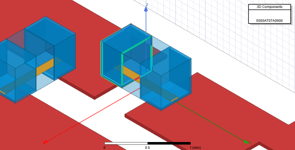
\includegraphics[width=3.5in]{images/brick_model.png}
        \caption{``Brick'' representation of capacitor package, note the one differential port shown as the orange rectangle parallel to the plane of PCB.} 
        \label{fig:brick_model}
        \end{center}
    \end{figure}
    
    \subsection{Versitility of Full-Wave Models: Simulation Example}
    Another limitation of equivalent circuit models is the fact that
    they are usually developed based on measurements made on a specific transmission line medium, and the values of some of the model's parasitics depend on the medium in which it was developed.
    Grounded Co-planar Waveguide (GCPW) has seen an increase in use for applications in the tens of GHz given the fact that it operates quasi-TEM up to higher frequencies than microstrip, as shown in Figure 2 of \cite{coonrod2012comparing}. 
    A geometric model used in conjunction
    with a full-wave electromagnetics simulator can give the engineer
    confidence that the component will act as predicted independent of medium.
    
     Similarly, researchers in the field of antenna design have also
    encountered the fact that a capacitor may not perform at the nominal
    capacitance if it is not in a traditional microstrip configuration. In
    \cite{mumcuCapacitors}, Figure 5b and 3b, measured data shows a 50 MHz shift
    downward in frequency which is in part attributable to the fact that
    an ideal, nominally-valued capacitor was used, with no modeling of the
    real component's interaction with the surrounding environment.
    
    The parasitic which has a value most sensitive to medium is the
    termination to ground capacitance, as is demonstrated by the circuit
    and full-wave simulations below.
    This will be accomplished through the addition of a simple network of L's and C's representing some of the parasitic effects corresponding to the outside of the capacitor, which are then fit to the responses of 3-D capacitor models situated in microstrip and GCPW.
    
     Pictured in Figure \ref{fig:mstrip_gcpw_designs} are two full-wave models of a 12 pF Johanson R14S
    capacitor, one mounted on a \(50 \Omega\) microstrip transmission line
    (W=1.647mm), the other mounted on a \(50 \Omega\) GCPW line (W=1.048mm, G = 0.2mm). Vias in the grounded co-planar waveguide medium are modeled by a strip of conductor with the same width as top and bottom metal, which extends from the top metal to the bottom metal through the substrate. Both models are a simulated 30 mil Rogers 4350B substrate, with $\epsilon_r$ = 3.66 and h=0.762mm. S-Parameters are simulated using a modal simulation setup, in a solution region extending the maximum dimension of the design by 100\% in either side in $\pm$ X, 200\% in $ \pm$ Z, with no offset in $\pm $ Y to facilitate wave ports. The use of wave ports enables the portion of transmission line leading up to the component to be de-embedded.
    
    	\begin{figure}[H]
			\begin{center}
			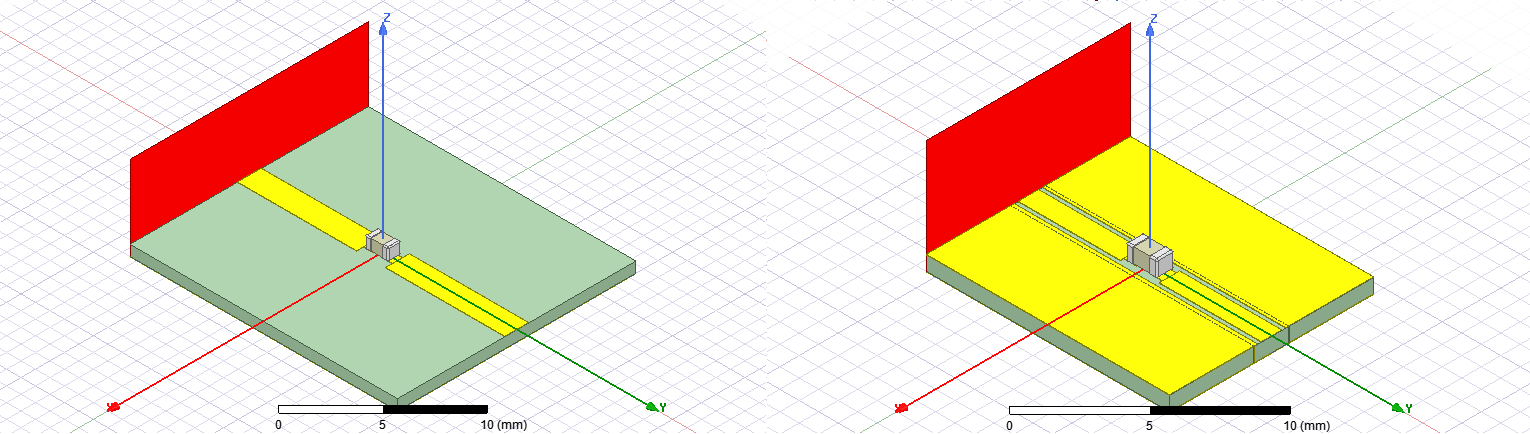
\includegraphics[width=6in]{images/mstrip_v_gcpw/hfss_designs.png}
			\caption{HFSS models of the Johanson R14S High Q Capacitor mounted on microstrip and grounded co-planar waveguide.} 
			\label{fig:mstrip_gcpw_designs}
			\end{center}
		\end{figure}
            
   
       From Figure \ref{fig:mstrip_gcpw_designs} ,we can see that if the termination to ground capacitance was going to change as a result of switching from Microstrip to GCPW, we would expect it to increase. An increase like this would be due to the ground now extending up to the top conductor of the circuit board through the vias, thus decreasing the distance between ground to the terminations, and thereby increasing the capacitance, as $ C = \frac{A\epsilon}{d}$ (very roughly) applies here. 
    
        A conceptual analysis of the response of the the two capacitors' return losses will reveal that the termination-to-ground capacitance does indeed increase. \(S_{11}\) of both capacitors for f = 0.01 to 20 GHz is plotted  in Figure \ref{fig:mstrip_gcpw_s11}. The self-resonance of the capacitor on microstrip is sharp and around 1.8 GHz, whilst the GCPW mounted capacitor's resonance is more gradual and at about 2.8 GHz -- a considerable shift, which anecdotally gives the impression that the same capacitor can be used up to a higher frequency using GCPW. 
        
        \begin{figure}[H]
			\begin{center}
			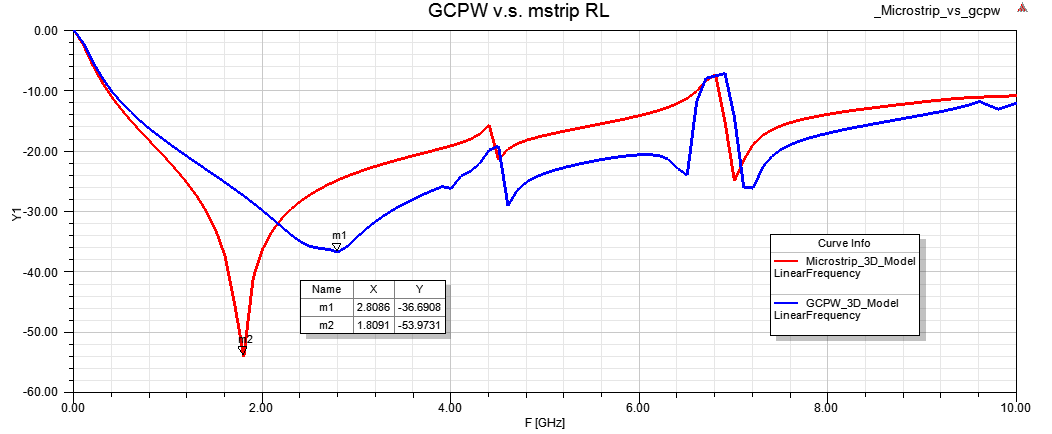
\includegraphics[width=6in]{images/mstrip_v_gcpw/S11.png}
			\caption{$S_{11}$ of the R14S capacitors mounted on microstrip and grounded co-planar waveguide --- note how the self-resonance of the component shifts upwards.} 
			\label{fig:mstrip_gcpw_s11}
			\end{center}
        \end{figure}

    We can now fit the response of these capacitors using a Modelithics Global equivalent circuit model in ``Simplified Parasitic Model'' mode, along with termination-and-pad-to-ground and termination-to-termination capacitance, and a series inductance associated with the pads and the terminations.
    The ``Simplified Parasitic Model'' mode, as discussed in section \ref{differential_port_explanation}, is a mode in which all of the parasitic effects associated with the terminations of the device are removed, leaving behind effects corresponding to the ``inside'' of the component, such as effective series resistance, inductance, and other parasitic capacitances.
            
        \begin{figure}[H]
			\begin{center}
			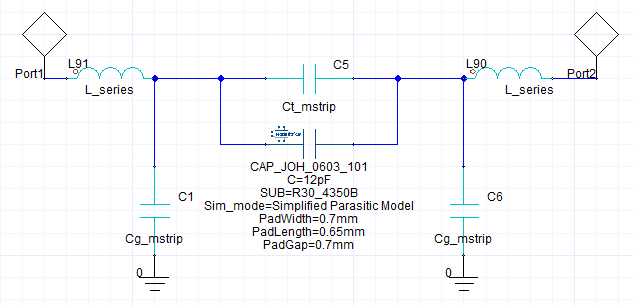
\includegraphics[width=5in]{images/mstrip_v_gcpw/parasitic_topology.png}
			\caption{Idealized circuit representation of parasitic effects corresponding to the package of the capacitor.} 
			\label{fig:mstrip_gcpw_parasitic_network}
			\end{center}
		\end{figure}

     Figure \ref{fig:mstrip_gcpw_parasitic_network} shows the circuit schematic in
     Nexxim, ANSYS' circuit simulator bundled alongside HFSS, in which it is
     possible to co-simulate the S-parameters of HFSS designs. This circuit will
     be fit against the response of the full-wave model mounted on microstrip by
     adjusting the values $L_{series}, C_{g,mstrip},$ and $C_{t,mstrip}$.
     The same topology was used to fit the response of the full-wave model on 
     grounded co-planar waveguide, with the same value of $L_{series}$ 
     corresponding to the termination inductance, but with different values 
     for the capacitances, $C_{g,gcpw},$ and $C_{t,gcpw}$.
        
    Comparing the circuit simulations and the HFSS simulations, the self resonance
    of the circuit simulation started out much higher than predicted by HFSS in the
    case of both microstrip and GCPW. Increasing the value of $L_{series}$ shifted
    both resonances downwards, and then increasing $C_g$ different amounts in 
    each the GCPW and microstrip cases shifted the resonances upwards to match the
    full-wave model.
	    
        \begin{figure}
            \centering
			    \begin{subfigure}{\textwidth}
                    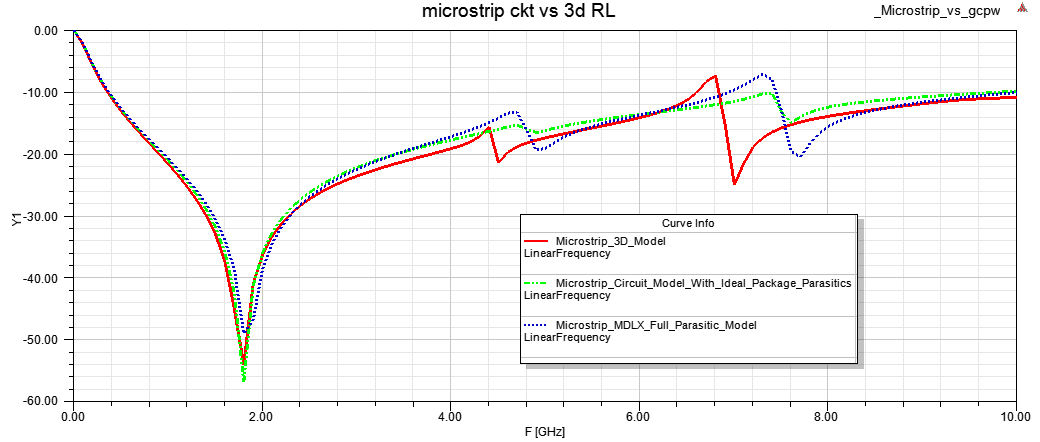
\includegraphics[width=\linewidth]{images/mstrip_v_gcpw/microstrip_comparison.png}
            \vspace{-\topsep}
            \begin{itemize}
                \centering
                \setlength{\parskip}{0pt}
                \setlength{\itemsep}{0pt} 
                \color{blue}
                \item Global equivalent circuit model developed for microstrip
                \color{red}
                \item Full-wave model on microstrip fixture
                \color{green}
                \item Global model in ``Simplified Parasitics Mode'' with simple termination parasitic network fit to microstrip
            \end{itemize}
            \vspace*{-9pt}
                    \caption{Fit responses on microstrip.}
                    \label{fig:mstrip_gcpw_comparisona}
                \end{subfigure}
                \hfill
			    \begin{subfigure}{\textwidth}
                    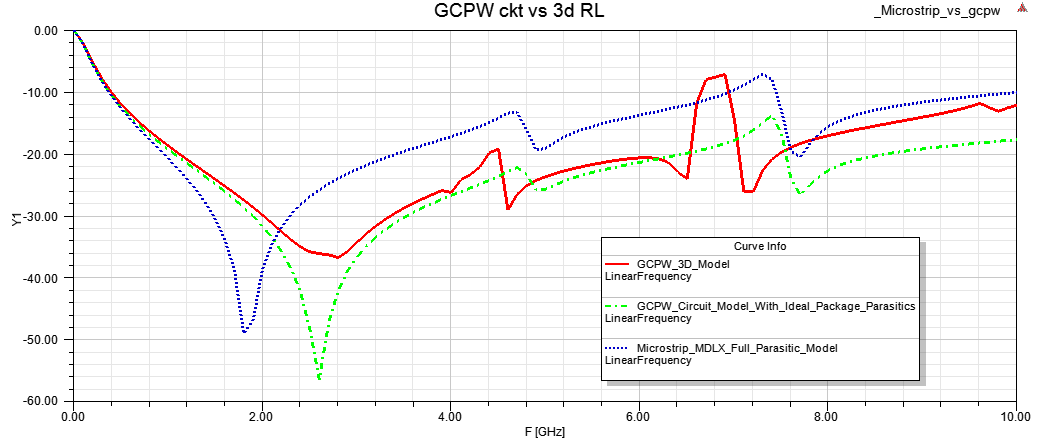
\includegraphics[width=\linewidth]{images/mstrip_v_gcpw/gcpw_comparison.png}
            \vspace{-\topsep}
            \begin{itemize}
                \centering
                \setlength{\parskip}{0pt}
                \setlength{\itemsep}{0pt} 
                \color{blue}
                \item Global equivalent circuit model developed for microstrip
                \color{red}
                \item Full-wave model on GCPW fixture
                \color{green}
                \item Global model in ``Simplified Parasitics Mode'' with simple termination parasitic network fit to GCPW
            \end{itemize}
            \vspace*{-9pt}
                    \caption{Fit responses on grounded co-planar waveguide.}
                    \label{fig:mstrip_gcpw_comparisonb}
                \end{subfigure}
		\end{figure}
		
		The values which produced these responses can be found in Table
		\ref{tbl:mstrip_gcpw_final values}
		
		\floatstyle{plaintop}
		\restylefloat{table}					
		\begin{table}[H]
		\centering
		\begin{tabular}{|c|c|}
			\hline
			  Component & Value \\
			 \hline
			 $L_{series}$ & 0.32 nH \\
			 \hline
			 $C_{g,mstrip}$ & 38.6 fF \\
			 \hline
			 $C_{t,mstrip}$ & 93.0 fF \\
			 \hline
			 $C_{g,gcpw}$ & 105.0 fF \\
			 \hline
			 $C_{t,gcpw}$ & 141.2 fF \\
			 \hline
		\end{tabular}
		\caption{Values of parasitic components.}
		\label{tbl:mstrip_gcpw_final values}
		\end{table}
		
			Thus we can see the considerable difference between the values of 
			parasitics in microstrip v.s. GCPW.  The availability of a validated 3-D EM model can allow these parasitics to be assessed without having two different equivalent circuit models, or conversely can assist with developing equivalent circuit models for specific situations without the need for additional configuration specific test fixtures and measurements. 
		
    \subsection{Concepts and Design Techniques}
    \subsubsection{Using Circuit Model Co-Simulation to Inform Gradient Descent}
    \label{cosimulation_inform_3D}
        Though there can be a considerable difference between the performance of circuit
    models and 3-D passive models as was discussed in the previous two sections, circuit models are still very useful for microwave design. 
    Furthermore, circuit models can be used in conjunction with 3-D models to greatly speed the full-wave design process. 
    Even in configurations in which the manufactured design is not represented well by equivalent circuit models, the combination of component values which give the best response in the full-wave simulator are more easily attainable by gradient descent from the optimum circuit values. 
    
    Consider the two circuit topologies in Figure \ref{fig:mn_ckt_reps}. 
    Shown are two L-section matching networks, both consisting of first a series C and then a shunt L, which are matching a load of 25 $\Omega$ to 50 $\Omega$. 
    In the \ref{fig:mn_ckt_reps} (a), only an ideal representation of the lumped elements is given. For the purposes of example, we'll say that \ref{fig:mn_ckt_reps} (b) is a more accurate version of the real matching network to be manufactured, and that it models two parasitic shunt capacitances to ground, both with a value of $C_p = 0.5 pF$. The idealized network (network A) and the more accurately simulated network (network B) are analogous to a network simulated with a circuit and full-wave representation of components respectively, as will be seen in later chapters. 
    
	\begin{figure}%
	    \centering
	    \subfloat[][Circuit representation of co-simulation]
	    {
			\begin{circuitikz}
              \draw
              (3,3) to [short,-o] (2,3)
              (3,3) to [C,l_=$C$] (6,3)
              (3,3) to [L,l_=$L$] (3,1)
              (6,3) to [R,l_=$25 \Omega$] (6,1)  
              (6,1) node[ground] {}  (6,1)  
              (3,1) node[ground] {} (3,1)
              ; 
             \end{circuitikz}
	    } %
	    \qquad
	    \subfloat[][Circuit representation of full-wave models with added parasitic capacitance]
	    {
			\begin{circuitikz}
              \draw
              (3,3) to [short,-o] (2,3)
              (3,3) to [C,l_=$C$] (6,3)
              (3,3) to [L,l_=$L$] (3,1)
              (3,3) to [C,l_=$C_p$] (3,5)
              (6,3) to [C,l_=$C_p$] (6,5)
              (6,3) to [R,l_=$25 \Omega$] (6,1)  
              (6,1) node[ground] {}  (6,1)  
              (3,1) node[ground] {} (3,1)
              (6,5) node[ground,rotate=180] {}  (6,5)  
              (3,5) node[ground,rotate=180] {}  (3,5)  
              ; 
             \end{circuitikz}
	    }
	    \caption{Equivalent circuit representations of co-simulated and full-wave match analysis, where $C_p$ is a parasitic capacitance of 0.5 pF.}%
	    \label{fig:mn_ckt_reps} %
    \end{figure} 
    
    Shown in Figure \ref{fig:2d_cost_visual} are surfaces representing how well matched to 50 $\Omega$ the impedances looking into the two networks are, with blue representing the \ref{fig:mn_ckt_reps} (a), and red representing \ref{fig:mn_ckt_reps} (b). The height of the surface corresponds to the dB magnitude of S11 when looking into one of the labeled networks, the X axis to inductance of the shunt inductor and likewise the Y axis to the capacitance of the series capacitor in both networks. 
    Figure \ref{fig:mn_ckt_reps} gives an intuition into an approximation that microwave designers often implicitly make when they move from less accurate to more accurate simulations. 
    Namely it is assumed that if the S parameters of network A and network B are given as:
        $$ S_a = f_a(L,C), \qquad S_b = f_b(L,C) $$ 
    Then we see in this example, and in many other instances when the accuracy of a simulation is improved that:
        $$ f_a(L + L_{diff},C+C_{diff}) \approx  f_b(L,C) $$ 
    which is certainly true in the case of \ref{fig:mn_ckt_reps}, where the return loss at the minimum or the surrounding areas for network B is essentially the same, and the entire response of the network is largely just shifted in terms of the component value needed.
    If the optimum values for network B are $L_b$ and $C_b$, and likewise the optimum values for network A are $L_a$ and $C_a$, as long as $L_a$ and $C_a$ lie in the basin of attraction with a minimum $L_b$ and $C_b$, then one is guaranteed convergence to $L_b,C_b$.
    A ``basin of attraction'' of a real-valued function $f(x)$ is the set of all $x$ for which:
    $$ \frac{d}{dt} x(t) = - \nabla f(x(t))$$
    converges to a particular $x_{min}$ as $t$ tends to infinity.
    
    This of course generalizes to any amount of components and respective values (or design parameters in general), and shows how reaching a point in this basin of attraction in the more accurate simulation is important to achieving a good design.
    Also, in the case of the gradient descent to be introduced in the next chapter, only the part values adjacent to the current point are tested, and thus a point close to the minimum desired is very important to the algorithm's timely completion. 
    
    Thus, the initial simulation of any network with circuit components is important to understanding the density of basins of attraction in the solution space (e.g. whether there are alternate, less optimal minima which one is in danger of optimizing to close by), and to provide a point in a basin of attraction in the more accurate simulation with a desired minimum. 
    Gradually increasing the accuracy of the simulation of a design from a theoretical staring point is often done in many simulation based workflows in part for these reasons, and using full-wave component models after circuit models is not an exception to this pattern.
    
    \begin{figure}[H]
		\begin{center}
        	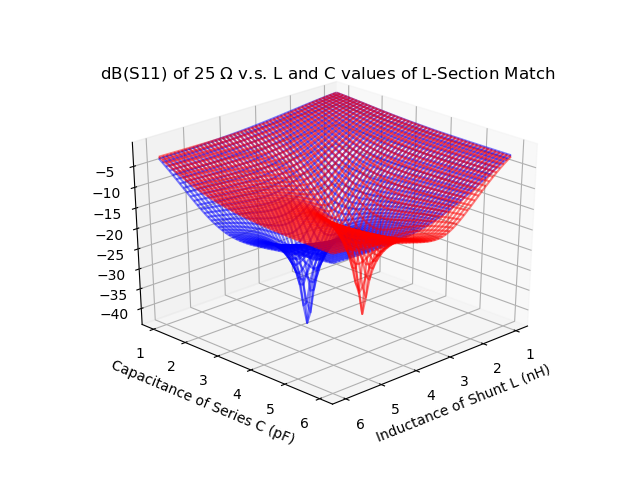
\includegraphics[width=\textwidth]{images/cosimulation_inform/match_surface_isometric.png} 
            \caption{S11 v.s. part value of series C and shunt L for Figures \ref{fig:mn_ckt_reps} (a) (blue) and (b) (red), f = 2 GHz.}
            \label{fig:2d_cost_visual}
		\end{center}
	\end{figure}
	
	\subsubsection{A Discrete Gradient Descent Algorithm for Finding Optimal Configurations of Part Values}
	
    While it is valuable to know that a design might act differently from a circuit simulation by performing an equivalent full-wave simulation, it is more useful to the designer to be able to adjust the design for these full-wave effects if design constraints necessitate that components are in an unusual configuration, or where they will interact.
    Assuming our circuit simulation has brought us into a basin of attraction in the 3-D model simulated cost function, we can use a gradient descent algorithm in order to obtain the minimum for the region.
    
    %algorithm
    Of course, since there is no analytic formulation of the cost v.s. the values of each of the components in the design, the gradient will have to be evaluated numerically.
    This can be done by taking a centered difference with respect to each of the variables in order to obtain a gradient of the cost. 
    Since in real life only certain discrete values for passive components are available, the algorithm used to demonstrate gradient descent with these components does not use the magnitude, and only steps in the direction of an increase rather than adjusting the size of the jump to the next iterate based off of the magnitude of the gradient. 
    The specific rules used by the algorithm are detailed at a high-level in \ref{fig:pseudocode}.
    
	\begin{figure}
    % \captionof{figure}[Discrete Part Value Gradient Descent (PseudoCode)]{Discrete Part Value Gradient Descent.}
    \begin{center}
    \begin{minipage}{.8\linewidth}
    \begin{algorithmic}[1]
        \Require {$x^{start},f(x)$}
        
        \State $x \gets x^{start}$ %\Comment{x is a list of indices for which component in the family to use in circuit.}
        \State $n \gets$ length$(x)$
        \While {True}
            \For {$i=0$ to $n$}
                \If{all $x_i$ at minimum }
                    \textbf{break}
                \EndIf
                \State $ x^{+} = [x_0,x_1,...,x_i + 1,...,x_n] $
                \State $ x^{-} = [x_0,x_1,...,x_i - 1,...,x_n] $
                \If {$f(x^{-}) < f(x) < f(x^{+})$}
                    \State $x \gets x^{-}$
                    \State no $x_i$ at minimum
                \ElsIf {$f(x^{-}) > f(x) > f(x^{+})$}
                    \State $x \gets x^{+}$
                    \State no $x_i$ at minimum
                \ElsIf {$f(x^{-}) > f(x)$ and  $f(x^{+}) > f(x)$}
                    \State $x_i $ at minimum
                \ElsIf {$f(x^{-}) < f(x)$ and  $f(x^{+}) < f(x)$}
                    \State raise warning %\Comment{Means solution surface isn't convex}
                    \If {$f(x^-) > f(x^+)$}
                        \State $x \gets x^{+}$
                    \ElsIf {$f(x^+) > f(x^-)$}
                        \State $x \gets x^{-}$
                    \EndIf 
                    \State no $x_i$ at minimum
                \EndIf 
            \EndFor
        \EndWhile
        \Return x,f(x)
    
        \caption{Discrete part value gradient descent pseudocode.}
        \end{algorithmic}
        \end{minipage}
        \end{center}
        \label{fig:pseudocode}
    \end{figure}
    \pagebreak

    %visualization
    With a discerning eye, one can reconcile the logic detailed above to the visualization of cost v.s. component combination values shown in \ref{fig:ant_mn_cost_visual}. 
    Each of the three axes in this visualization correspond to the index of an inductor value for a 3-inductor tee topology match, as is shown in Figure \ref{fig:2450_mdlx_ckt_cosim}. 
    The color, as explained by the bar on the right side of Figure \ref{fig:ant_mn_cost_visual}, corresponds to how well-matched each combination of 3 inductor values (represented by a point in 3-D space) is. 
    With this in mind, one can recognize the "star" pattern and subsequent selection of a neighbor that is done by the algorithm (as can be seen happening at the point labeled ``Optimum Circuit Model Match'').
    Also observable is the algorithm finding a minimum, as is shown at the point labeled ``Lowest Cost-3-D Modeled Point'', where all the neighbors of said point have higher costs. 
    
    \begin{figure}[H]
		\begin{center}
        	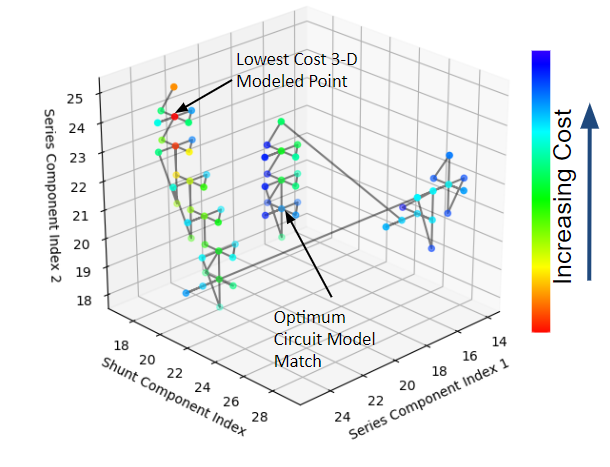
\includegraphics[width=\textwidth]{images/gradient_descent/grad_descent_visual.PNG} 
            \caption{Visualization of Cost v.s. inductor values of 3-inductor tee-section match.}
            \label{fig:ant_mn_cost_visual}
		\end{center}
	\end{figure}
	
    %implementation
    This is not the most sophisticated local search algorithm, but simply serves as a proof of concept that optimization on full-wave components is very useful and can be implemented in commercial simulation software.
    The specifics of how the algorithm was implemented can be seen in Figures \ref{fig:grad_desc_implementation} and \ref{fig:grad_desc_cost_calc}.
    All code was written for this purpose in IronPython 2.7 which has good integration with ANSYS HFSS, and is available upon request. 

    \begin{figure}[H]
		\begin{center}
        	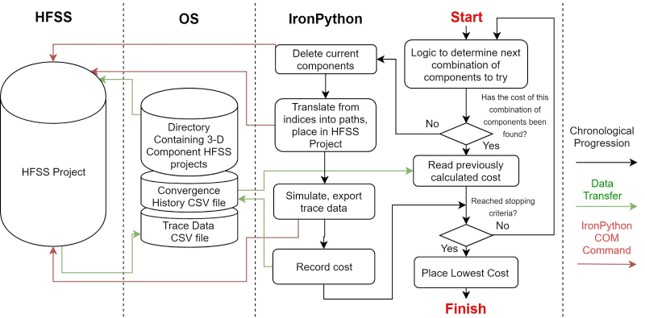
\includegraphics[width=\textwidth]{images/gradient_descent/flowchart.png} 
            \caption{Flowchart detailing implementation of 3-D geometry optimization algorithm.}
            \label{fig:grad_desc_implementation}
		\end{center}
	\end{figure}
	
    \begin{figure}[H]
		\begin{center}
        	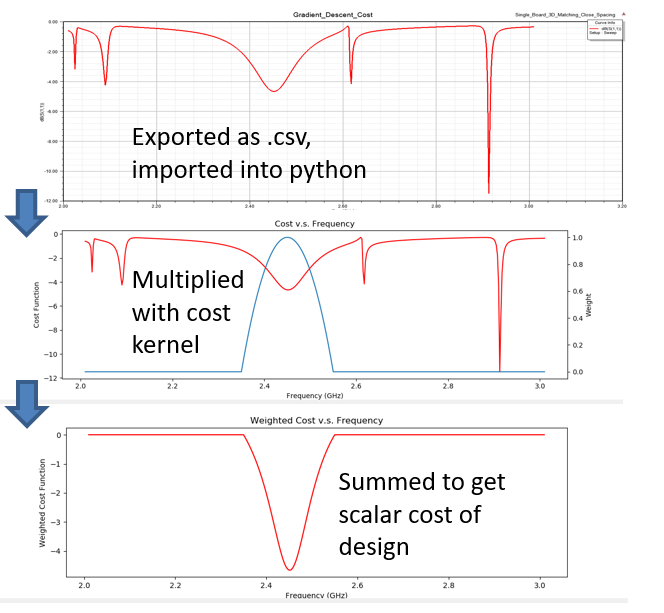
\includegraphics[width=\textwidth]{images/gradient_descent/cost_calculation.PNG} 
            \caption{How cost is determined from results of HFSS simulation}
            \label{fig:grad_desc_cost_calc}
		\end{center}
	\end{figure}

    \subsection{Summary}
    In this chapter, what is to be achieved is detailed, and relevant literature to the problem is given. 
    Additionally, the commercial models for circuit simulator, full-wave simulator, and hybrid brick models were introduced.
    Finally, the philosophy behind the design flow to be used is presented, as well as the workings of the gradient descent algorithm used throughout Chapter 3.
        
    % summarize the first chapter
	
%%%%%%%%%%%%%%%%%%%%%%%%%%%%%%%%%%%%%%%%%%%%%%%%%%%%%%%%%%%%%%%%%%%%%%%%%%%%%
% Inter Component-Coupling
    \usfchapter{AN INVESTIGATION INTO INTER-COMPONENT COUPLING}
    
     \indent Inter-component coupling is present to some degree in circuits at all
    frequencies, and is widely understood in a conceptual sense. This kind
    of coupling is the added response caused by putting two or more
    components together, that would not be present when the components are
    on their own. Physically, this corresponds to the mutual capacitance
    or inductance between the outer parts of two components.
    
        It is intuitive that these effects are more pronounced when
    components are closer together, but the effect of other factors such as the substrate thickness, relative rotation of components, and the size of the component, have not been systematically studied in the literature. 
    In this chapter, A full-factorial analysis of the effect of case size, component type, distance, and relative angle on coupling as previously defined is presented. 
    \subsection{Background and Definition of Inter-Component Coupling}
    
    \subsubsection{Design of Experiments Terms and Concepts}
    One way to investigate whether and to what degree these different properties change the response of the network is by conducting a Design of Experiments (DOE) analysis: a systematic way of investigating the effect of certain variables on a response in a statistically supported fashion. 
    
    A common type of such an experiment is the factorial experiment -- an experiment in which two or more ``factors'' are varied, and their effect on a ``response variable'' are studied.
    In our case, the relevant factors are component type, size, distance, and mutual angle, and the response variable is the amount of S-parameter error observed.
    Factorial experiments are a generalization of simpler, one-factor-at-a-time experiments in which a trial is carried out at every combination of the ``levels'', or values, of the factors of interest. 
    This improves greatly upon studying each of the effects separately: More information is received per trial, and the effect of ``interactions'' are taken into account. 
    An interaction between factors is said to occur when  one factor that effects the response variable is dependent on the level of another factor. 
    Figure \ref{fig:interaction_example} shows an example of such an interaction, from \cite{interaction_example}, which used a factorial design to study the effects of temperature and UV exposure on fish infection rates. 
    As one can see in the chart, if someone had designed individual experiments studying the effects of temperature and UV exposure on infection, they would not have seen the huge increase in whitespots, a metric of the severity of infection, that occurs when ``both'' the temperature and UV exposure are higher.  
    
    \begin{figure}[H]
		\begin{center}
        	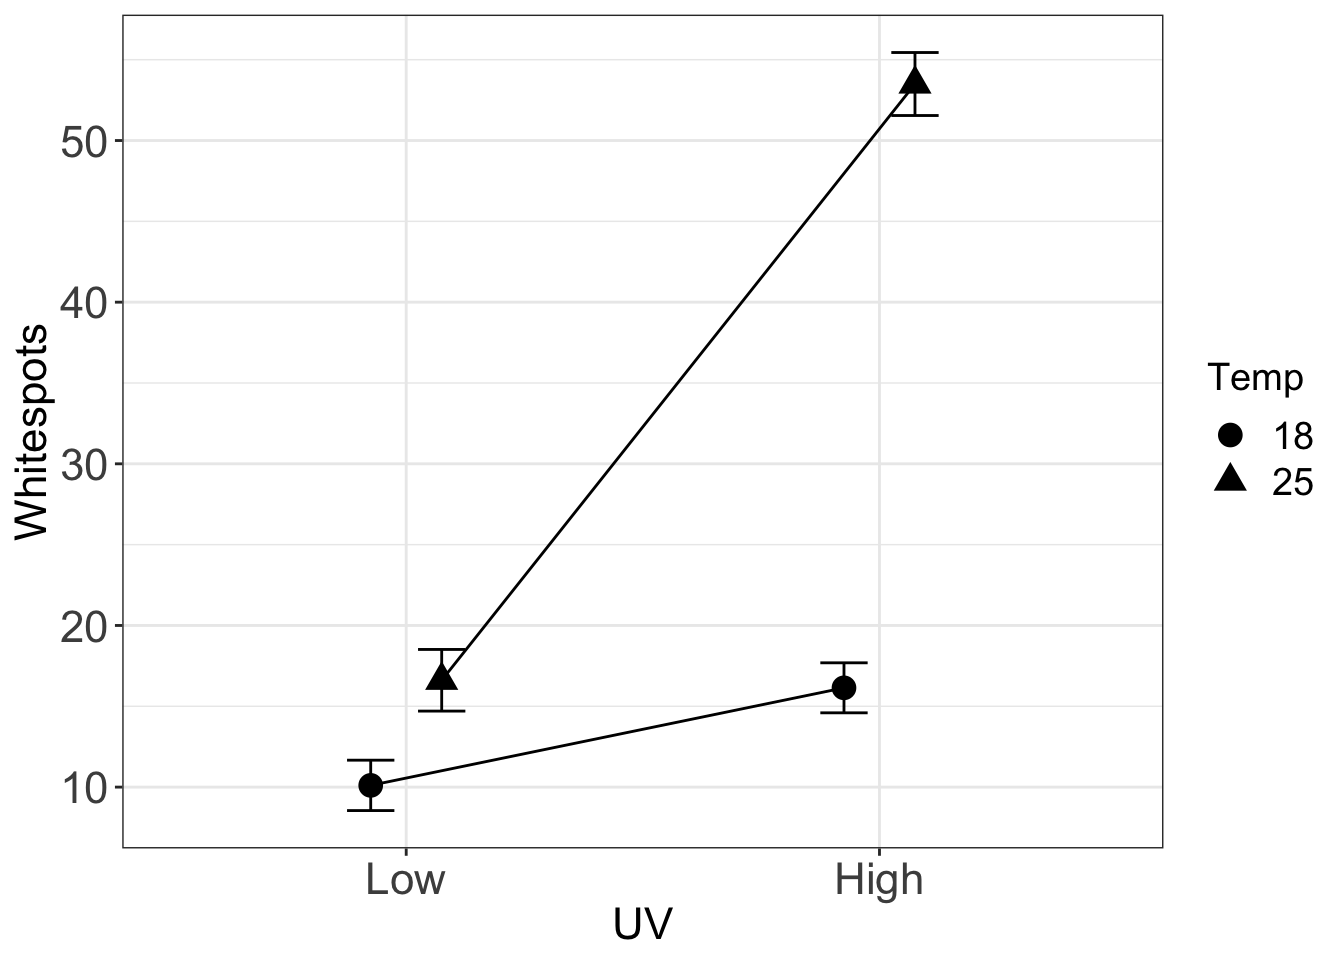
\includegraphics[width=4.5in]{images/ANOVA/gg_interaction-example-1.png} 
			\caption{A plot showing interaction between temperature and UV exposure in their effect on number of whitespots. } 
			\label{fig:interaction_example}
		\end{center}
	\end{figure}    
    
    
    
       If coupling is to be studied in an experiment, we must first have a
    measurement-based mathematical formulation of coupling. The following
    section shows the metric which will be used to measure coupling in this study.

    \subsubsection{Wave Cascade Matrices}
    All microwave engineers are familiar with S parameters, which are commonly collected into a matrix in the case of two-port networks. 
    The S matrix relates the incident (or \(a\)) waves to the reflected (or \(b\))
    waves as follows:
    \begin{gather}
     \begin{bmatrix} b_1 \\ b_2 \end{bmatrix}
     =
      \bar S 
      \begin{bmatrix} a_1 \\ a_2  \end{bmatrix}
    \end{gather}
    
    Less widely used, but very convenient for finding the response of cascaded two-port microwave networks is the wave cascade matrix, \(\bar W\). 
    This relates the incident and reflected waves of a two-port network like so:
    
    \begin{gather}
     \begin{bmatrix} b_1 \\ a_1 \end{bmatrix}
     =
      \bar W 
      \begin{bmatrix} a_2 \\ b_2  \end{bmatrix}
    \end{gather}
    
       From this we see that the wave cascade matrix of two two-port
    networks cascaded is \(\bar W_1 \bar W_2\) , where $\bar W_1$ and $\bar W_2$
    are the wave cascade matrices of arbitrary two ports 1 and 2.
    This nomenclature to describe cascading two-ports is used in the next section as part of the definition of coupling.
    
    \subsubsection{Coupling Metric}
    Consider a design composed of \(k\) cascaded two-port networks as shown below:
        
    \begin{figure}[H]
        \centering
          \begin{circuitikz}
              \draw [dotted] (-2,0) -- (0,0);
              \draw [dotted] (2,0) -- (4,0);
              \draw 
              (-4,0) to[twoport,t=$W_1$,o-o] (-2,0) 
              (0,0) to[twoport,t=$W_i$,o-o] (2,0)
            % TODO add ellipsis 
                
              (4,0) to[twoport,t=$W_k$,o-o] (6,0) ; 
            %   \node at (-1,0) {$\cdots$}
            \end{circuitikz}
    		\caption{Network consisting of \(k\) cascaded 2 port networks.} 
    		\label{fig:cascaded_2ports}
	\end{figure}   
	
    If \(i\) is the variable which indexes these cascaded two-port networks, we define the \(i^{th}\) two-port's wave cascade matrix as \(\bar W_i\), and the wave cascade matrix of the entire network is \(\bar W_{tot}\).
    The S-parameter matrices for the same networks, \(\bar S_i\) and \(\bar S_{tot}\), will have to be directly measured in order to find coupling by this metric.
    Since the measurement of \(\bar S_{tot}\) will have all of the sub-designs directly adjacent to each other, there will be some amount of coupling between the components.
    This requires measurements of the complete design, as well as each individual sub-design.
    So, we can define a coupling of a specific ordered set of two-port designs to be:
    $$\text{Coupling} = \sum_{i=1}^{2}\sum_{j=1}^{2} \left|\left( \bar S_{tot} - \text{W\_to\_S}\left(\prod_{i=1}^k \bar W_i \right)\right)[i][j]\right|$$ 
    if W\_to\_S is a function which takes a wave-cascade matrix and returns an equivalent S-parameter matrix.
    
    In words, the coupling metric in question is the sum of the magnitudes of all the differences in S-parameters between the measured total circuit and it's individual parts cascaded. 
    This will be the coupling metric referred to alternately by ``Coupling and S-paramter error'' throughout the rest of the text. 
    
    \subsubsection{Change in Series Resonant Frequency as a Metric}
    
    Another metric which captures how much a design has changed is the change in the first Series Resonant Frequency, referred to later in the text solely as SRF. 
    The series resonant frequency is the frequency at which capacitive parasitics dominate the response of an inductor, or when inductive parasitics dominate the response of a capacitor. 
    At this point, a dip can be seen in the magnitude of the S21 of a capacitor, and the same dip can be observed in the magnitude of the S11 of an inductor. 
    Since this is the point where the component stops having it's intended response, this frequency is very related to the usable frequency range of a design in which these components are used.
    For this reason, the ability to predict this frequency is an important quality for a model, and so, the difference in this frequency was also calculated between the measured and re-cascaded networks.
    
    \subsection{Methodology}
    Given what was previously discussed, a series of designs and sub-designs were manufactured with the goal of investigating coupling as a function of the previously mentioned factors. 
    
    
    \subsubsection{Independent Variables Investigated} 
    
    The independent variables, known as treatments in the context of a statistical experiment, were chosen to be the things most likely to influence the degree of coupling a circuit exhibits given the authors experience and intuition. A table of all of the treatments used in the design and their respective levels is given in Table 2.
    
    \begin{table}[H]
        \begin{center}
            \begin{tabular}{|l|l|l|l|}
            \hline
            Treatment & Level 1 & Level 2 & Level 3\\
            \hline
            Component Type & Capacitor & Inductor & \\
            \hline
            Component Size & 0402 & 0201 & \\
            \hline
            Distance & .5 mm & 1.0 mm & 1.5 mm\\
            \hline
            Angle & 0° & 45° & 90°\\
            \hline
            \end{tabular}
        	\caption{Factors and associated levels to be used in factorial design.}
        \end{center}
        \label{tbl:treats}
	\end{table}   
	
    ``Component Type'' refers to whether the components were inductors or capacitors.
    The capacitors used for this design were from the Johanson R05L and R07S families for the 0201 and 0402 case sizes respectively.
    TDK MLG0603S chip inductors were used for the 0201 case size, and MHQ1005 for the 0402 size.
    These specific parts were chosen as they had a relatively low tolerance, and had the internal geometry most similar to each other as possible while having different case sizes.
    It was hypothesized that the inductors would exhibit more coupling than capacitors, as the E field lines begin at one plate of a capacitor and end at the other, meaning the majority of the field that electrical energy is stored in would seem to be entirely contained within the component.
    Conversely, solenoid inductors like the chip inductors in question store their energy in a magnetic field which continues out of the top and bottom of the package, allowing for more interaction with the environment. 
    
    ``Component Size'' refers to the case sizes of the aforementioned parts.
    Two component sizes were tested in the study, 0402 and 0201 imperial.
    It was hypothesized that having a larger case size would increase the amount of coupling between two components, with the idea that increasing the size of a termination would be akin to increasing the size of a capacitor plate.
    
    ``Angle'' describes the angle each is offset from the horizontal axis of the interconnect.
    It was predicted that increasing this angle would increase the coupling.
    Test fixtures with all treatments held constant except are shown as the left two test fixtures in Figure \ref{fig:treatment_explanation},
    
    ``Distance'' for this study was defined in two ways: Interconnect distance, and center distance.
    As can be seen in Figure \ref{fig:treatment_explanation}, the interconnect distance is the length of the interconnect as shown in red, and the center distance is the distance between the center of the parts, shown in blue.
    Changing the angle changes the center distance, so to investigate this from a physical perspective or with the intent to build a model, this would be the value of the treatment one should use.
    From a circuit design perspective however, a designer is able to find the ``interconnect distance'' as defined here much easier to use these results as a rule of thumb, and allowed the creation of the test designs to be straightforward. 
    Considering these two things the resultant data is processed using both interconnect and center distance.
    As one might surmise, decreasing the distance between the components was expected to increase coupling, and be the most strongly related to changing coupling.
    
    \begin{figure}[H]
		\begin{center}
        	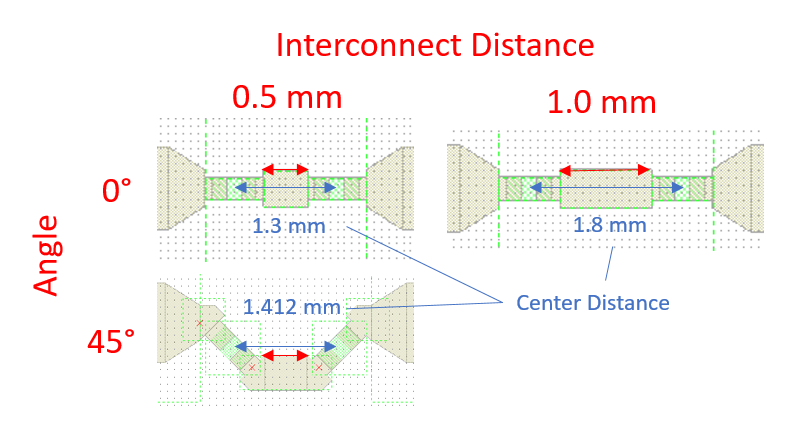
\includegraphics[width=\textwidth]{images/ANOVA/treatment_explanations.png} 
			\caption{Test fixtures showing how angle and distance was varied, as well as labeling interconnect and center distances.} 
			\label{fig:treatment_explanation}
		\end{center}
	\end{figure}    
	
    \subsubsection{Controlled Factors, Manufacture and Measurement} 
    Additional factors, such as the effect of microstrip v.s. GCPW media and substrate height on coupling  were considered for investigation, but ultimately not studied due to time and cost constraints.
    The problem of what part value to use was also the object of much deliberation -- it was not immediately obvious what combination of inductor and capacitor values would produce the most even comparison.
    Controlling for the Series Resonant Frequency (SRF) between the inductors and capacitors seemed to be the most logical decision, as this would control for the portion of the band in which the components were operating normally.
    Part value was considered as a factor, but since the utility of this experiment was imagined to be for a designer with an existing topology and circuit values trying to minimize the effect of interaction, so treatements relating to the geometric properties of a design remained the focus.
    
    All designs were manufactured on 20 mil Rogers 4350B substrate, and were manufactured in a board house using lithography to etch the conductors and electroplating to form the vias.
    Boards were populated by hand, which did incur a bit of variation in the exact placement of the components.
    The designs were measured from  45 MHz to 9 GHz using a $Z_0$ corrected multiline TRL calibration, and probed using 650 $\upmu$m coaxial probes. % TODO cite
    
    \begin{figure}[H]
		\begin{center}
        	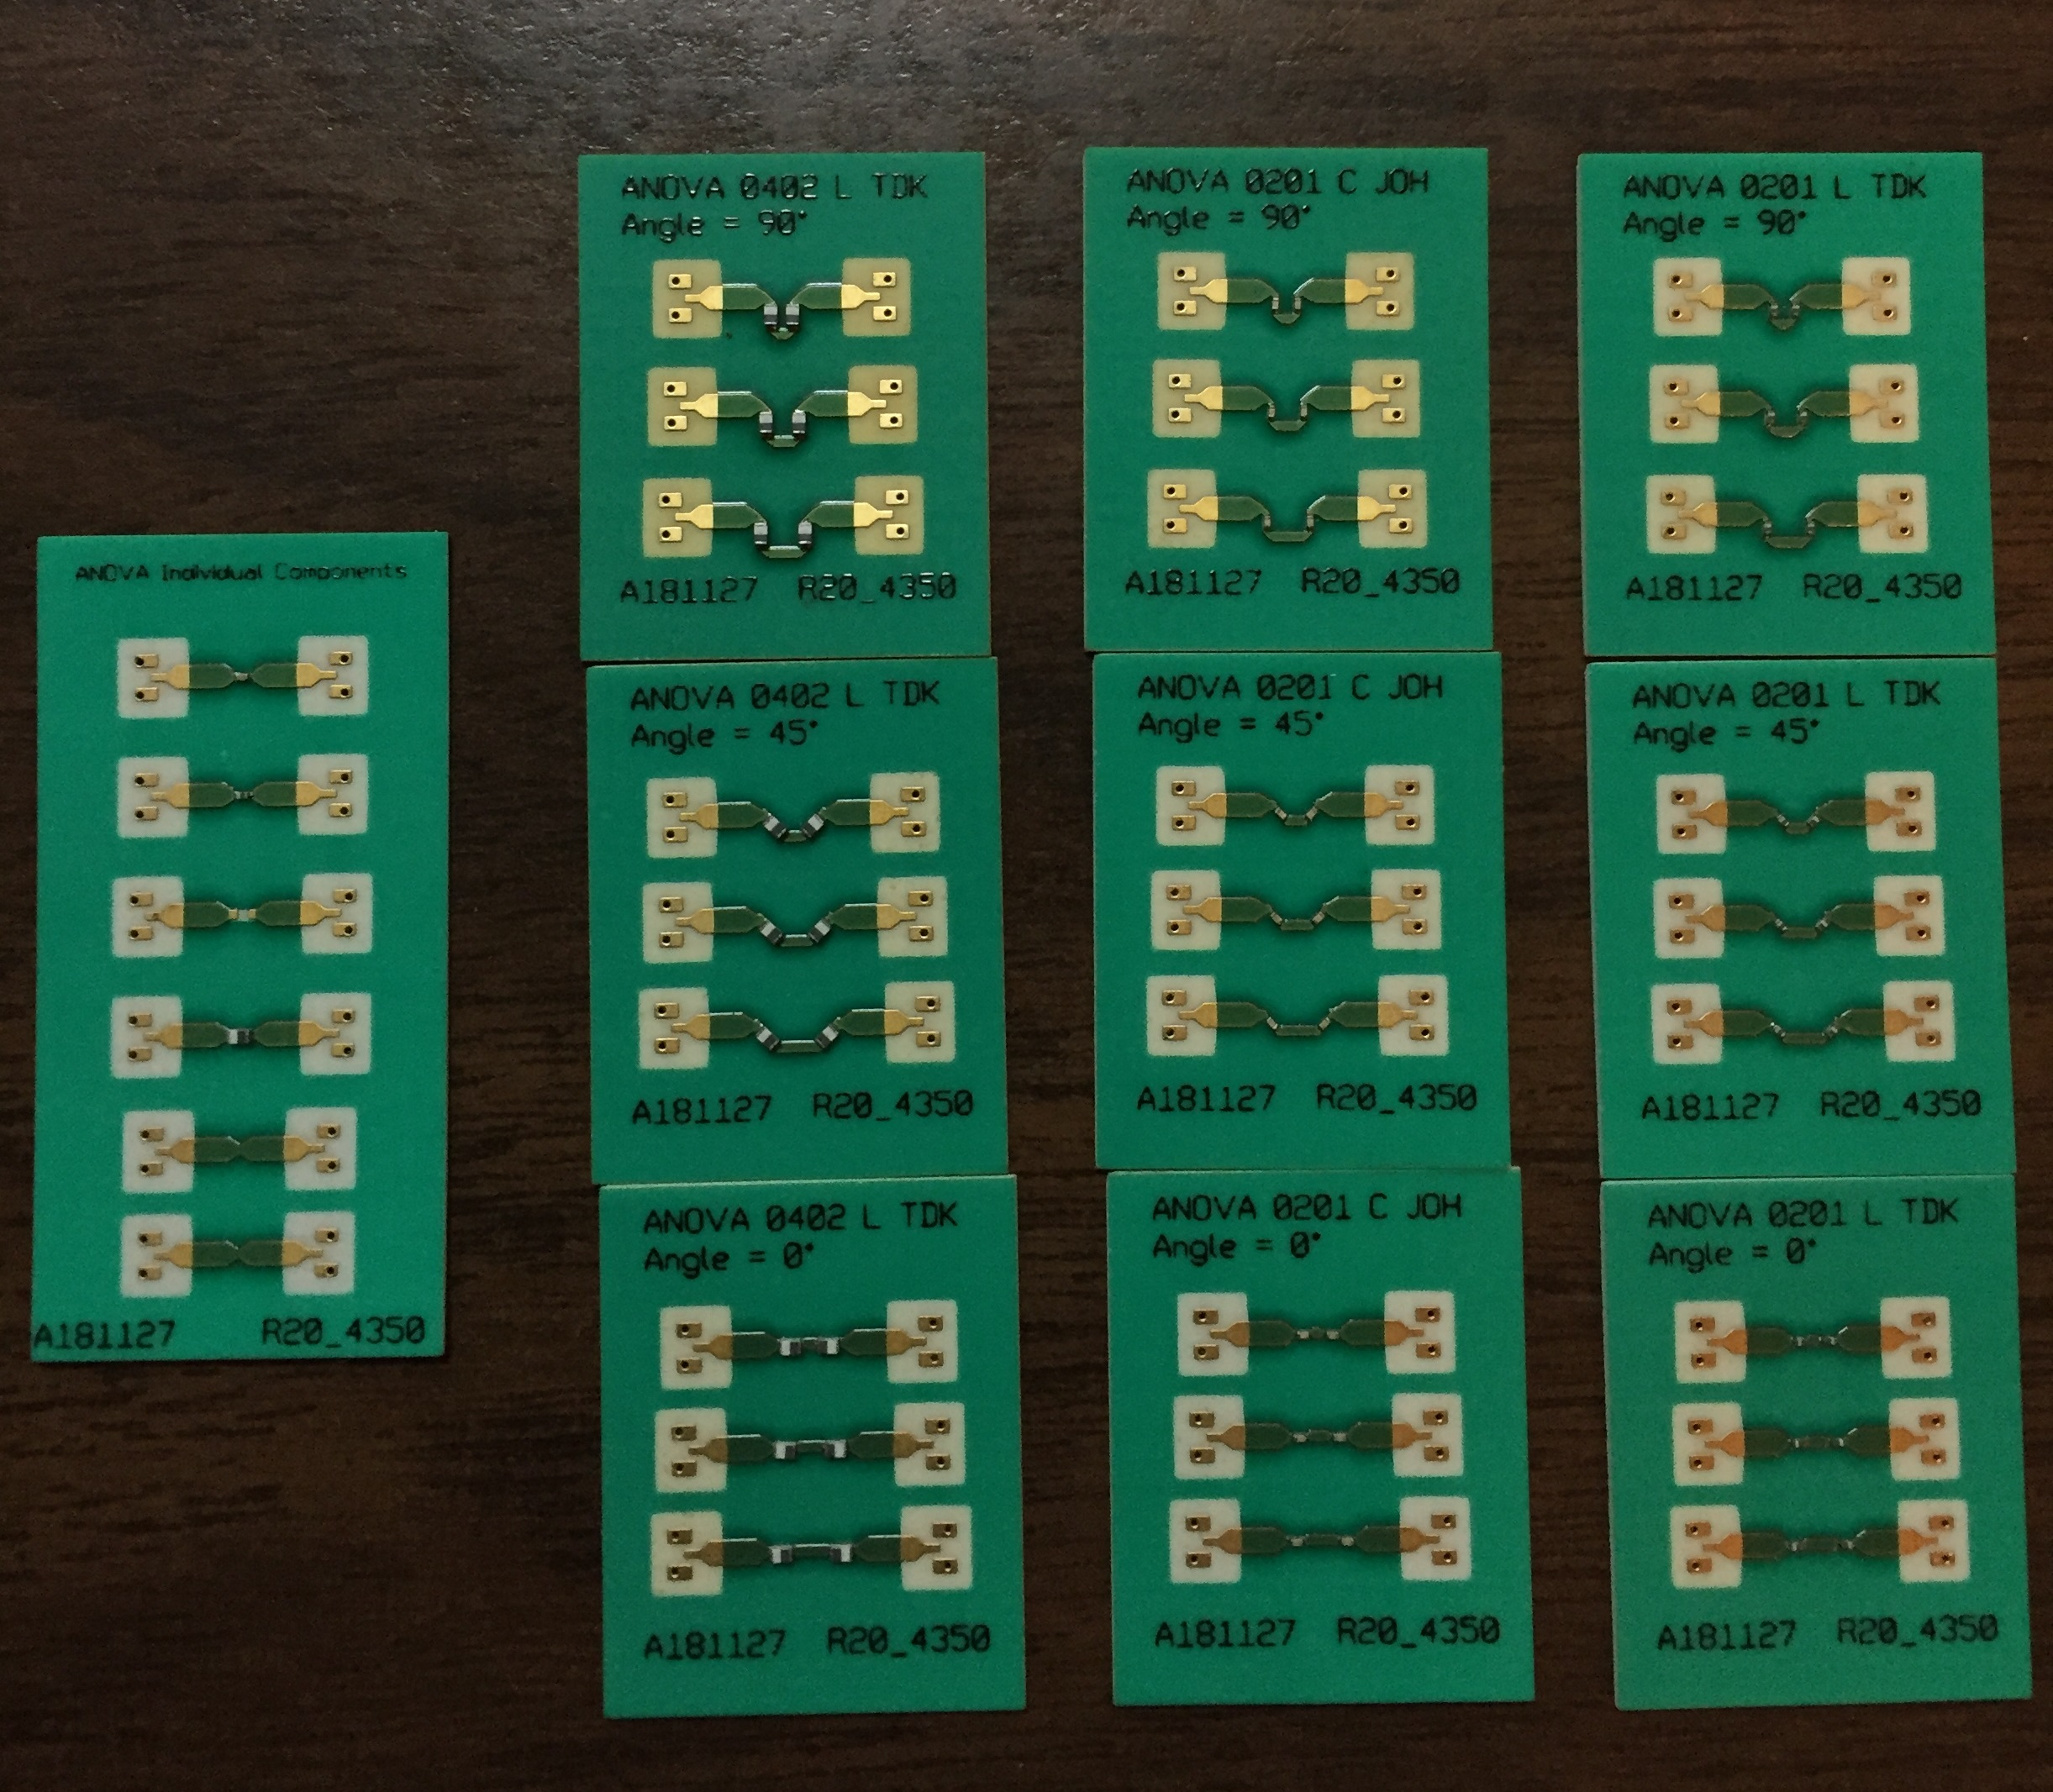
\includegraphics[width=4in]{images/ANOVA/manufactured_test_fixtures.jpg} 
			\caption{10 of the 15 manufactured boards.} 
			\label{fig:test_fixtures_irl}
		\end{center}
	\end{figure}    
    
    As mentioned previously, a measure of coupling is taken by cascading individual measured parts of a specific design and comparing to a measurement of the manufactured complete design. This was done using AWR's Microwave Office circuit simulator. 
    
    \begin{figure}[H]
		\begin{center}
        	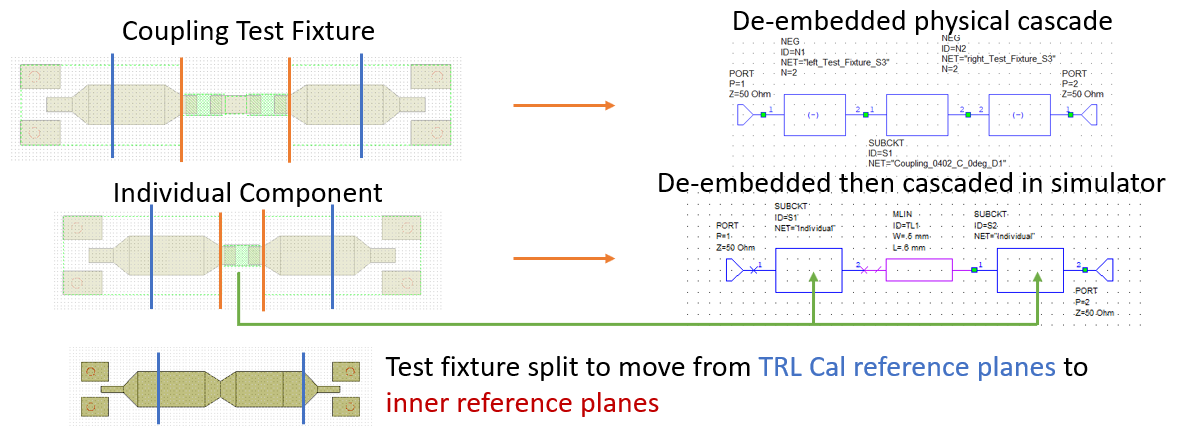
\includegraphics[width=\textwidth]{images/ANOVA/cascasde_vs_physical_explanation.png} 
			\caption{How physically and mathematically cascaded sub-designs were compared.} 
			\label{fig:cascading}
		\end{center}
	\end{figure}    
	
	Due to the limited number of boards able to be manufactured, the interconnects were simulated instead of being measured. 
	This was done by tuning the substrate parameters for a 2D method of moments simulation of the test fixture thru (pictured in the bottom of \ref{fig:cascading}) until an excellent fit was achieved. 
    The difference between the actual response of these sub-networks and the simulated response is an error which confounds the response in question, but the since the difference between the simulated test fixture and the measured test fixture response was less than the variation between samples, the error should be insignificant compared to the effect we are trying to measure.
    
    % TODO cite skrf 
    All 36 of the simulated responses were exported, and the coupling metrics were calculated between them using `sckikit-rf`, an open-source python library for microwave engineering --- more about this software can be found at www.scikit-rf.org.
	The metrics were recorded to a file and analyzed with Minitab, a commercial software used for analyzing statistical experiments, from which most of the plots in the remainder of this chapter were generated.
	
    \subsection{Results}
    The values for S-parameter error, and change in SRF versus the factors of case size, component type, angle, and distance, are shown in Table 3 below.
    All of the figures, statistical analyses and subsequent conclusions were drawn from this data.

    \begin{table}
    \centering
        \begin{tabular}{|r|r|r|r|r|l|l|}%
        
        \hline
        Case\_Size&Is\_Ind&Angle\_deg&Distance\_mm&Center\_Dist&Coupling&SRF\_Delta\_GHz \\
        \hline
        0&0&0&0.5&1.3&46.55&-0.012 \\
        \hline
        0&0&0&1&1.8&54.60&-0.005 \\
        \hline
        0&0&0&1.5&2.3&41.47&0.008 \\
        \hline
        0&0&45&0.5&1.42&57.44&0.005 \\
        \hline
        0&0&45&1&1.92&59.49&-0.106 \\
        \hline
        0&0&45&1.5&2.42&49.49&-0.122 \\
        \hline
        0&0&90&0.5&1&89.70&-0.177 \\
        \hline
        0&0&90&1&1.5&80.21&-0.242 \\
        \hline
        0&0&90&1.5&2&73.00&-0.188 \\
        \hline
        0&1&0&0.5&1.3&83.83&0.116 \\
        \hline
        0&1&0&1&1.8&171.11&0.204 \\
        \hline
        0&1&0&1.5&2.3&66.72&0.061 \\
        \hline
        0&1&45&0.5&1.42&166.50&0.189 \\
        \hline
        0&1&45&1&1.92&85.61&0.044 \\
        \hline
        0&1&45&1.5&2.42&98.54&0.05 \\
        \hline
        0&1&90&0.5&1&165.39&0.135 \\
        \hline
        0&1&90&1&1.5&139.14&0.091 \\
        \hline
        0&1&90&1.5&2&89.54&0.023 \\
        \hline
        1&0&0&0.5&1.7&40.01&0.111 \\
        \hline
        1&0&0&1&2.19&37.53&0.163 \\
        \hline
        1&0&0&1.5&2.7&30.10&0.119 \\
        \hline
        1&0&45&0.5&1.7&92.65&0.219 \\
        \hline
        1&0&45&1&2.18&58.15&0.061 \\
        \hline
        1&0&45&1.5&2.7&56.53&0.152 \\
        \hline
        1&0&90&0.5&1&252.19&0.595 \\
        \hline
        1&0&90&1&1.5&159.89&0.363 \\
        \hline
        1&0&90&1.5&2&130.37&0.248 \\
        \hline
        1&1&0&0.5&1.7&112.42&0.067 \\
        \hline
        1&1&0&1&2.19&87.99&0.052 \\
        \hline
        1&1&0&1.5&2.7&79.90&-0.062 \\
        \hline
        1&1&45&0.5&1.7&71.71&0.049 \\
        \hline
        1&1&45&1&2.18&80.81&0.083 \\
        \hline
        1&1&45&1.5&2.7&69.64&-0.079 \\
        \hline
        1&1&90&0.5&1&201.69&0.159 \\
        \hline
        1&1&90&1&1.5&62.61&0.009 \\
        \hline
        1&1&90&1.5&2&60.12&0.060 \\
        \hline
        \label{tbl:anova_data}
        \caption{Data resulting from measuring ANOVA test fixtures and analyzing data}
        \end{tabular}
    \end{table}

    A general overview of the effects of each of the treatments on each of the responses can be seen in Figures \ref{fig:main_effects_coupling} and \ref{fig:main_effects_abs}. 
    Note that in these plots, the interconnect distance is used instead of the center distance in order to maintain consistency between all of the factors and to provide a better visual indication of the effect of increasing distance.
    These plots, labeled ``Main Effects'', show the average value of the response for all trials which fall into the category labeled on the X axis.
    Categorical levels are represented as integers in Minitab, so for the ``Case\_Size'' factor, 0 corresponds to an 0201 component, and 1 corresponds to an 0402 component. 
    Similarly, for ``Is\_Ind'', 0 means that the component was a capacitor, and 1 for an inductor.
    For example, in \ref{fig:main_effects_coupling}, we see that corresponding to the 0 level of the ``Is\_Ind'' factor, the average S-parameter error was a little more than 75, and S-parameter error was more than 105 for the 1 level. 
    This means that the average S-parameter error of all of the inductors was about 30 more than that of the capacitors, giving us intuition into what effect the distinct levels of a factor are having on a response. 
    Though the absolute value of the S-parameter error may not have significance, this difference between the two averages can be compared to the variance in this response of each group to conclude with a specific certainty that the factor has an effect on the response.
    These charts also may give insight into the value of a factorial design as an efficient way of investigating many effects - since each of the trials was performed with a different combination of levels, we have the option of looking at many ``cross-sections'' of the data. 

    In Figure \ref{fig:main_effects_coupling}, the main effects for S-parameter error are shown. 
    As can be seen in the plot, case size did not seem to have too pronounced of an effect relative to the other factors. 
    The factor ``Angle\_deg'' for this plot should be thought of more like the product of angle and center distance, as though this shows the average S-parameter error was more for test fixtures having a 90 degree mutual angle, the center distance was also closer.
    Since this product does not have the same slope as the interconnect distance however, one can surmise that there is an additional increase in S-parameter error due to increase in angle between components.
    % TODO add reference to pareto charts
    The true effect that angle has on S-parameter error will be shown rigourously in the Pareto charts later in this chapter. 

    \begin{figure}[H]
		\begin{center}
            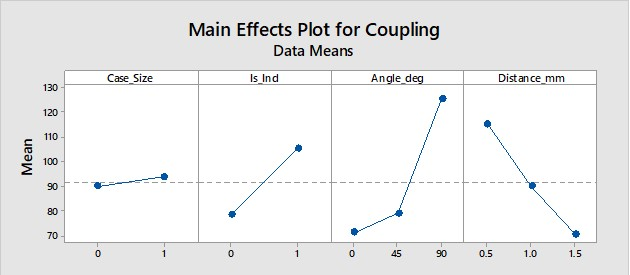
\includegraphics[width=\textwidth]{images/ANOVA/CouplingMainEffects.jpg} 
            % TODO figure out how to reference section?
			\caption{Main effects of factors on the S-parameter error as defined in ``Coupling Metric''.} 
			\label{fig:main_effects_coupling}
		\end{center}
    \end{figure}    

    Figure \ref{fig:main_effects_abs} displays the impact of the same factors in the absolute value of the change in SRF, measured in GHz. 
    Comparing this to \ref{fig:main_effects_coupling} generates questions, and some insight.
    First, the fact that ``Angle\_deg'' and ``Distance\_mm'' show a consistent shape in the response versus level is a good indicator that both responses are representative of the idea of inter-component interaction, and reinforces the idea that the factors are having the effect shown in both plots.
    Despite this, the effect of the categorical factors of the type and size of the component were not consistent between the responses. Where having an inductor instead of a capacitor increased the S-parameter error in Figure \ref{fig:main_effects_coupling}, here an inductor decreases the change in the SRF. 
    Likewise, having a larger case size did not affect the S-parameter error much, but did increase the change in SRF. 
    These differences can be reconciled by considering what kind of differences the two metrics quantify.
    In short, the S-parameter error will capture more changes than the change in SRF will. and is generally more sensitive than the change in SRF.
    Both S-parameter error and change in SRF are sensitive to changes in where resonances occur, but the S-parameter error may show things like discretions in phase that would not be accounted for by shift in SRF. 
    
    % TODO Changing from 90 degrees to 45 has bigger effect on coupling than simply spacing
    
    
    
    \begin{figure}[H]
		\begin{center}
        	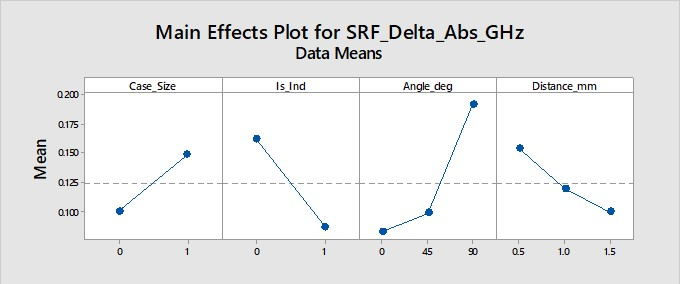
\includegraphics[width=\textwidth]{images/ANOVA/AbsSRFDeltaGHz.jpg} 
			\caption{Main Effects of factors on the absolute value of the change in SRF.}
			\label{fig:main_effects_abs}
		\end{center}
    \end{figure}    

    %%%%%%%%%%%%%%%%%%%%%%%%%%%%%%%%%%%%%%%%%%%%%%%%%%%%%%%%%%%%%%%%%%%%%%%%%%%%%%%%
    % BREAKING DOWN BY CAPACITORS AND INDUCTORS
    %%%%%%%%%%%%%%%%%%%%%%%%%%%%%%%%%%%%%%%%%%%%%%%%%%%%%%%%%%%%%%%%%%%%%%%%%%%%%%%%

    % \qquad Also shown in Figures \ref{fig:L_main_effects} and \ref{fig:C_main_effects} are factorial analyses of capacitors and inductors respectively which show the effects of interaction per component.
    % These plots better represent the behavior of these devices ove

    % \begin{figure}[H]
	% 	\begin{center}
    %     	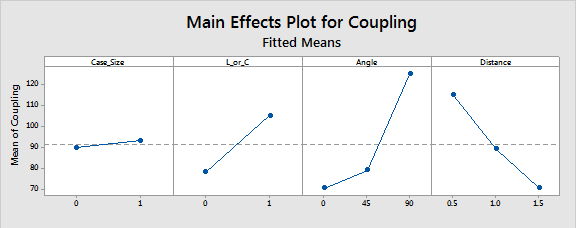
\includegraphics[width=\textwidth]{images/ANOVA/Main_effects.png} 
	% 		\caption{Main effects of factors using the interconnect distance} 
	% 		\label{fig:L_main_effects}
	% 	\end{center}
    % \end{figure}    
    
    % \begin{figure}[H]
	% 	\begin{center}
    %     	\includegraphics[width=\textwidth]{images/ANOVA/C_main_effects.png} 
	% 		\caption{Main effects of factors using the interconnect distance} 
	% 		\label{fig:C_main_effects}
	% 	\end{center}
    % \end{figure}    

    \subsubsection{Statistically Significant Effects}
    % TODO Pareto plots and interpretation 
    One useful reason for performing a factorial design is to try and draw conclusions about which factors affect the response and to what degree. 
    With this information, one can take special cares to ensure that a factor that the response is sensitive to is controlled, and prevent wasted effort by not excessively controlling factors that the response isn't sensitive to.
    Figures \ref{fig:pareto_coupling}  and \ref{fig:pareto_abs_srf} show the statistically significant effects on the S-parameter error and absolute value of change in SRF  respectively.
    Each one of the bars represents the certainty with which that specific term (or product of terms) affects the response, and the red line in the center of the graph represents the point at which you can say with 95\% certainty that the term in question has an effect (either increasing or decreasing) on the response. 
    The factors that consistently had a statistically provable impact on the response were, in order of aggregate significance: Angle, Case\_Size*Is\_Ind, Angle*Is\_Ind, and Is\_Ind.
    Though the reader may be surprised to not see distance as a significant factor for the S-parameter error, this is explained by the fact that the interconnect distance is used in this specific analysis.
    Angle, which is certainly significant as per these charts, is still confounded with distance.
    
    
    \begin{figure}[H]
		\begin{center}
        	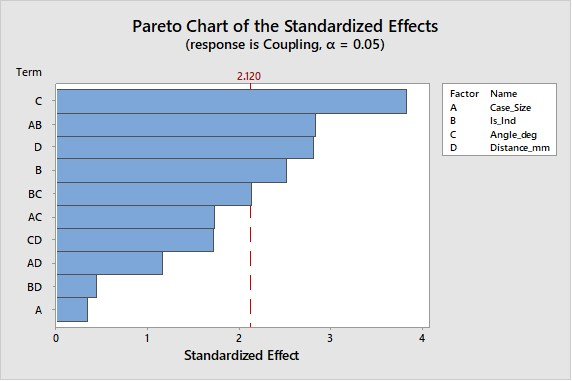
\includegraphics[width=0.7\textwidth]{images/ANOVA/pareto_coupling.jpg} 
			\caption{Pareto plot of S-parameter error v.s. treatments and interactions.} 
			\label{fig:pareto_coupling}
		\end{center}
    \end{figure}    

    \begin{figure}[H]
		\begin{center}
        	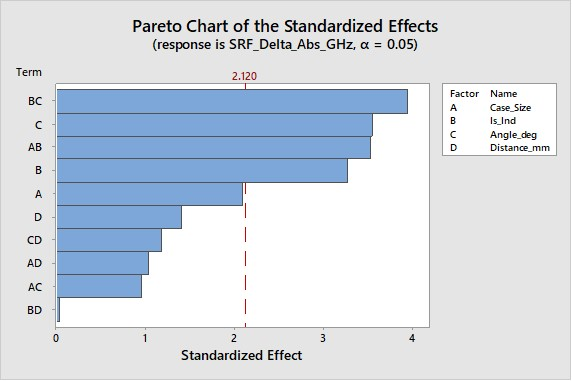
\includegraphics[width=0.7\textwidth]{images/ANOVA/pareto_abs_srf.jpg} 
			\caption{Pareto plot of absolute value of change in SRF v.s. treatments and interactions.} 
			\label{fig:pareto_abs_srf}
		\end{center}
    \end{figure}    

    A good visualization of this is in \ref{fig:minitab_model_visualization}, where one can see that the closest center distance occurs only occurs at the 90 degree angle level. 
    Following this, the fact that angle is very significant but not distance is revealing that there is an interaction between angle and distance. 
    This will be expanded upon in the next section.
    
    Another interesting result of these two plots is the fact that so many two factor interactions are present between inductors and the other factors.
    What can be concluded from these is that having components very close and directly alongside one another is especially bad when the components are inductors.
    This effect has a clear physical basis: mutual inductance beginning to occur between the two components.
    Since this idea is consistent with the main effects of the change in SRF, it was one of the reasons this metric was chosen as the response which would be fit by a behavioral model later in this chapter.
    
    \subsubsection{Interaction}
    
    Interaction matrices are another tool which can give insight into the meaning of two-factor interaction. 
    With our expectations built from the Pareto charts, we know where to look for effects like interaction, and also we can see whether the significant terms increase or decrease the value of the response.
    As demonstrated in \ref{fig:interaction_example} and the corresponding explanation, an interaction can be seen between nicely between angle and whether the component was an inductor as shown in Figure \ref{fig:interaction_abs_delta_srf}, and to a lesser degree in \ref{fig:interaction_coupling}. 
    For Figures \ref{fig:interaction_abs_delta_srf} and \ref{fig:interaction_coupling}, one must be careful when interpreting the right most column. 
    Though the factor that each individual colored line varies with is the center distance which is more physical, each individual data point is still at a different angle which is also a factor of interest, and is only the average over whichever factors remain when the factor represented by the change in line color is removed.
    
    To illustrate this point, the highest red point in the top right plot of Figure \ref{fig:interaction_abs_delta_srf} in only an average value between the two different components which shared a corner distance of 1mm and a 0402 case size.
    Contrast this with the leftmost chart, where the highest red point is an average of the 9 components which were 0402 capacitors.


    \begin{figure}[H]
		\begin{center}
        	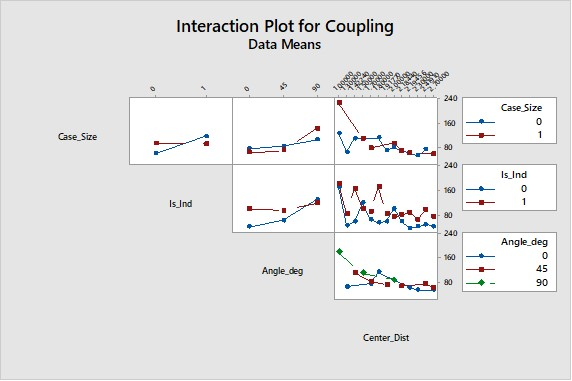
\includegraphics[width=0.8\textwidth]{images/ANOVA/interactions_coupling.jpg} 
			\caption{Interaction matrix using center distance for S-parameter error.} 
			\label{fig:interaction_coupling}
		\end{center}
    \end{figure}    
    
    \begin{figure}[H]
		\begin{center}
        	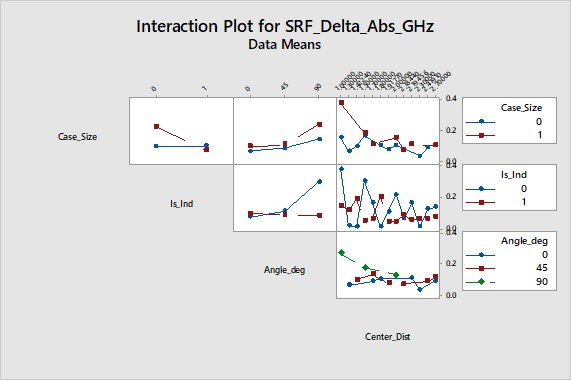
\includegraphics[width=0.8\textwidth]{images/ANOVA/interactions_abs_delta_srf.jpg} 
			\caption{Interaction matrix using center distance for absolute change in SRF.} 
			\label{fig:interaction_abs_delta_srf}
		\end{center}
    \end{figure}    


    % TODO interaction plots and interpretation
    \subsection{Design Implications}

    \subsubsection{Coupling Behavioral Model}
    One outcome from this study which could be of interest to a designer is the behavioral model produced of the absolute value of the shift in SRF between cascaded and measured responses of the test fixtures. 
    One model was developed each for the capacitors and the inductors, since all of the other factors are either interval (distance, angle) or ordinal (case size).
    Consistent with this thinking, distance, angle and case size are all inputs to the model. 
    This section will first go over the development and thinking behind the model, then the model will be presented. 

    The first model of absolute SRF shift that was investigated was the linear model as produced by Minitab, a simple linear model for each case size and component type. 
    This model is shown in Figure \ref{fig:minitab_linear_models}, and was found to be lacking for a couple of reasons. 
    First, the concavity of the surface measured was such that the linear failed to model the data properly within the bounds of the measured data. 
    Additionally, the behavior of the linear model outside the bounds of the measured data was clearly not physical.
    
    These qualities are shown graphically in Figure \ref{fig:minitab_model_visualization}, where one can see how the linear model compares to the measured data.
    As made clear in the title, this was the case for which ``Case\_Size'' as seen in \ref{fig:minitab_linear_models} had a value of 1, and for which ``Is\_Ind'' had a value of 0. 
    One can clearly see that the model needs more terms, or preferably a different response rather than a simple, no-interaction linear model. 
    The squares of all the errors in this case summed to 0.69.

    \begin{figure}[H]
		\begin{center}
        	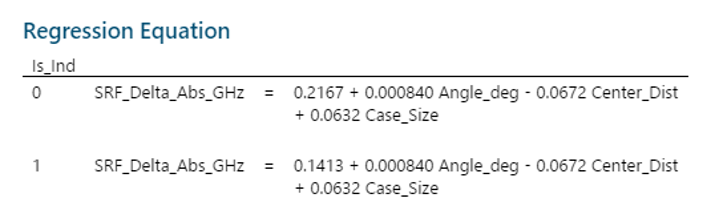
\includegraphics[width=\textwidth]{images/ANOVA/linear_models.png} 
			\caption{Initial linear regression explored as a guideline for coupling.}
			\label{fig:minitab_linear_models}
		\end{center}
    \end{figure}    
    
    \begin{figure}[H]
		\begin{center}
        	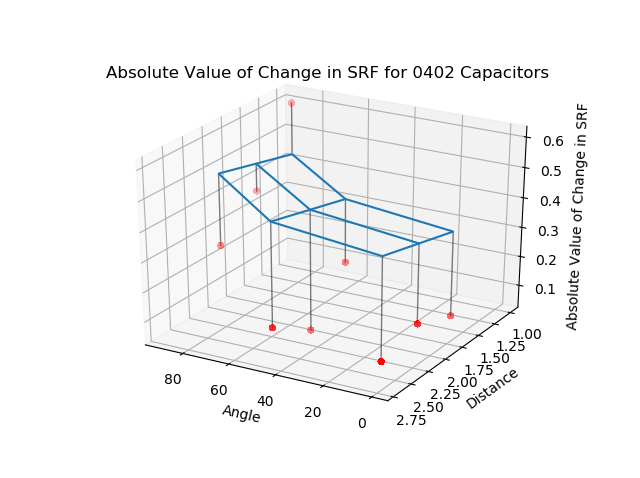
\includegraphics[width=\textwidth]{images/ANOVA/linear_model_surface.png} 
			\caption{3-D visualization of simple linear model v.s. measured data: red dots show measured data, the blue mesh shown is the model, and the black lines show the residual between the two. }
			\label{fig:minitab_model_visualization}
		\end{center}
    \end{figure}    

    At this point the shape of the data, as well as the physical basis for coupling was considered in the model. 
    An inverse relationship with distance was used as, if the measurements are proper, as distance approaches infinity, the interaction between the components should decrease to zero.
    Contrast this to a linear model, where after a zero crossing the absolute value of the change in SRF would actually begin to increase again. 
    The quadratic shape which the surface has in the direction of angle was determined by inspection and does not have a well-behaved end behavior similar to distance as only angles from 0 to 90 degrees make sense considering the definition of the angle as it was presented earlier.
    Equation \label{eq:individual_model} was fit to the measured data and then graphed using a least-squares regression in Python. 
    This model seems to fit the data well, and does not seem to be overfit considering the fact that there only two tuned parameters for 9 data points. 
    Using this model, the sum of the squares of the residuals for each case size and component type (tabulated in Table 4) was reduced at least an order of magnitude from the 0.69 given by the linear model.
    % TODO introduce model form
    \begin{equation}\label{eq:individual_model}
    \|\Delta SRF\| = \frac{c1 \cdot angle^2+ c0}{distance}
    \end{equation}
    
    
    \begin{figure}[H]%
	    \centering
	    \subfloat[][0402 Capacitor]{ 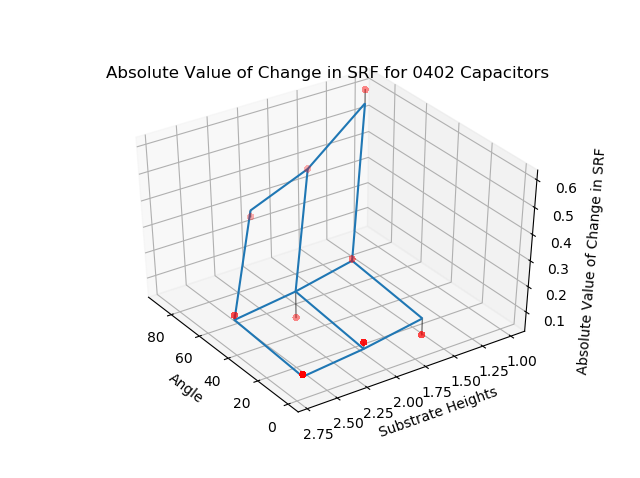
\includegraphics[width=0.5\textwidth]{images/ANOVA/cap_fit_srf_0402_zero_offset.png}  } %
	    \subfloat[][0201 Capacitor]{ 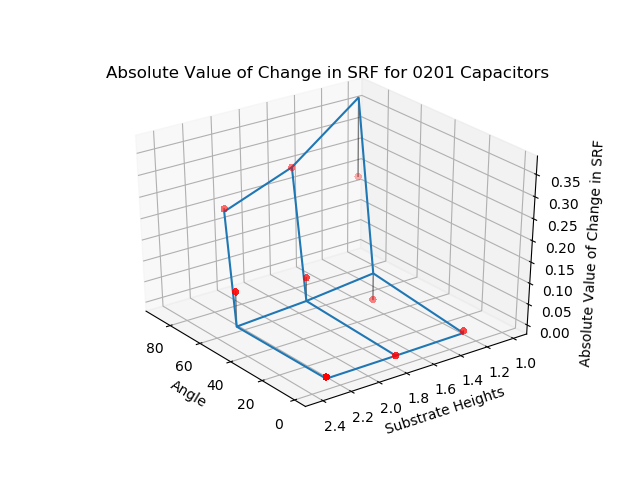
\includegraphics[width=0.5\textwidth]{images/ANOVA/cap_fit_srf_0201_zero_offset.png}} %
	    \break
	    \subfloat[][0402 Inductor]{ 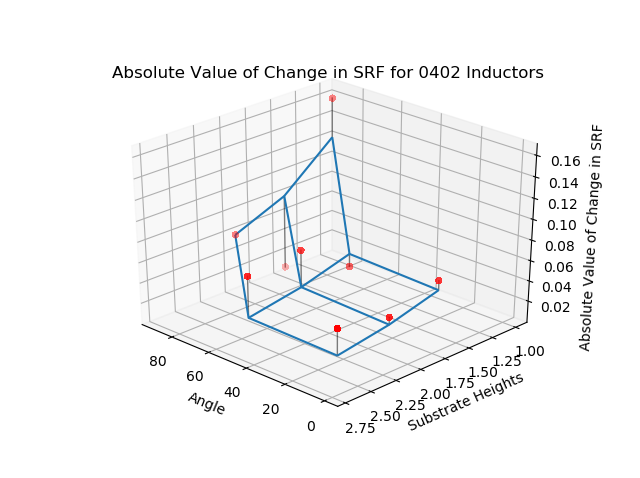
\includegraphics[width=0.5\textwidth]{images/ANOVA/ind_fit_srf_0402_zero_offset.png}  } %
	    \subfloat[][0201 Inductor]{ 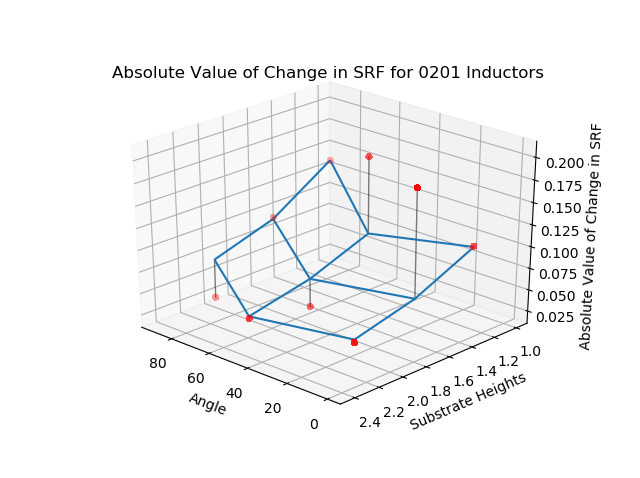
\includegraphics[width=0.5\textwidth]{images/ANOVA/ind_fit_srf_0201_zero_offset.png}} %
	    \caption{Data and model fit to absolute value of change in SRF for conditions given in each subcaption, using the new model form.}%
	    \label{fig:new_model_vis} %
    \end{figure} 
    
    \begin{table}[H]
        \begin{center}
            \begin{tabular}{|l|l|l|l|l| }
            \hline
            & 0201 C & 0402 C & 0201 L & 0402 L\\
            \hline
             c1 & 4.37E-5 & 3.03E-5 & 6.8E-5 & 2.7E-6\\
            \hline
            c0 & 0.01 & 0.3 & 0.08 & 0.1  \\
            \hline
            SSR & 0.049 & 0.019 & 0.025 & 0.01\\
            \hline
            \end{tabular}
            \label{tbl:individual_model_coeffs}
        	\caption{Model coefficients and associated errors for each type and size of component, where SSR stands for the sum of squares of residuals. }
        \end{center}
	\end{table}   
	
	Following the development of the per case size and component type models, the model was joined across case size, which is a relatively interval factor. 
	Since both capacitance and mutual inductance vary with the area of a surface or coil respectively, $c1$ and $c0$ of Equation \ref{eq:individual_model} was made to vary with the square of the length of the case in mils. 
	Note that this assumes that change in SRF varies directly with change in the ``amount of capacitance/inductance'' and is likely only a good approximation for a short while outside of teh verified case sizes.
	Consistent with the form seen in Equation \ref{eq:combined_model}, for capacitors and inductors $d3, d2, d1$ and $d0$ were chosen such that:
    \begin{equation*}
	c1_{0201} = d3 \cdot (20)^2 +d2, \qquad  c1_{0402} = d3 \cdot (40)^2 +d2 
    \end{equation*}
	and,  
    \begin{equation*}
    c0_{0201} = d1 \cdot (20)^2 +d0, \qquad  c0_{0402} = d1 \cdot (40)^2 +d0
    \end{equation*}
	
	In this manner, Equation \ref{eq:combined_model} below may additionally be extended to other case sizes. 
	It should be noted that the likelihood of this equation predicting change in SRF probably falls off rapidly as one deviates from the verified case sizes. 
	With Equation \ref{eq:combined_model}, a designer can define an acceptable shift in design frequency, then plug in the relevant parameters of the design they are working with in order to predict whether a shift due to coupling would be in an acceptable range.
	
    \begin{equation}\label{eq:combined_model}
   \|\Delta SRF\| = \frac{\left( d3\cdot case\_size^2 + d2 \right)\cdot angle^2 + \left( d1\cdot case\_size^2 + d0 \right)}{distance}
    \end{equation}
	
    \begin{table}[H]
        \begin{center}
            \begin{tabular}{|l|l|l|}
            \hline
            Coefficient Value & Capacitors & Inductors \\
            \hline
             d3 & -1.12E-8 & -3.42E-6 \\
            \hline
            d2 & 4.81E-5 & 8.17E-6  \\
            \hline
            d1 & 1.67E-4 & 1.67E-5 \\
            \hline
            d0 & 3.33E-2 & 7.33E-2 \\
            \hline
            \end{tabular}
            \label{tbl:model_coeffs}
        	\caption{Values of coefficients for the model form including case size given in \ref{eq:combined_model}}
        \end{center}
	\end{table}   
	
    The effect of coupling is also predicted reasonably well when investigated with the brick model of the Johanson R07S family of capacitors as is shown in Figure \ref{fig:anova_3d} below.
	    
    \begin{figure}[H]
		\begin{center}
        	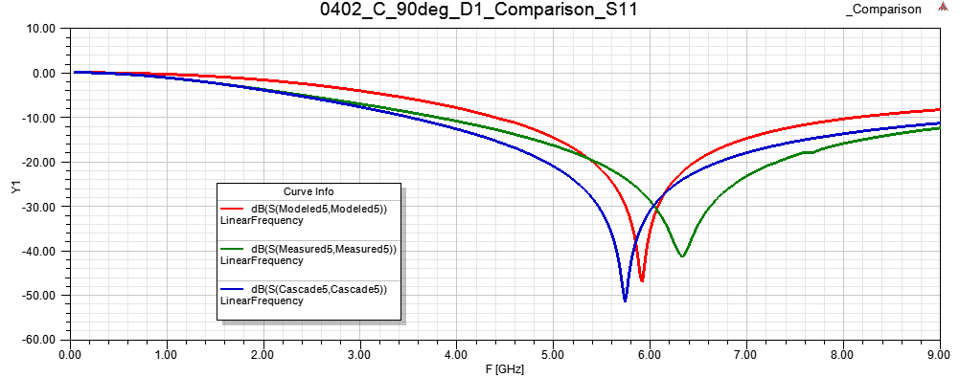
\includegraphics[width=\textwidth]{images/ANOVA/3D_model_fit.png} 
            \vspace{-\topsep}
            \begin{itemize}
                \centering
                \setlength{\parskip}{0pt}
                \setlength{\itemsep}{0pt} 
                \color{red}
                \item Brick Model Response
                \color{green}
                \item Directly Measured Response
                \color{blue}
                \item Cascaded Measured Response
            \end{itemize}
            \vspace*{-9pt}
			\caption{Response of 3-D model v.s. measured and re-cascaded capacitor coupling fixture.}
			\label{fig:anova_3d}
		\end{center}
    \end{figure}    

    \subsubsection{Arranging Lumped Elements to Avoid Coupling}
    % TODO example design
    % practical implications for designers
    The information obtained in the following sections is only valuable when put into the context of circuit design using lumped elements.
    In keeping with this idea, a couple of guidelines for laying out passive components in a context close to that of this study (microstrip on a 20 mil PCB with an $\epsilon_r$ of 3.66).
    
    In order to show how these results might inform layout of lumped elements on a PCB, a layout for a tee topology band pass Chebyshev filter was developed as seen in Figure \ref{fig:better_layout}. 
    Figure \ref{fig:better_layout} (a) shows how one might layout a filter with this topology without considering component interaction.
    Mirroring how the ideal components might have been drawn in a schematic presenting this topology, this was synthesized without taking into account a couple of considerations that would help save board real estate and reduce the chance that the response will be different than expected.
    Notice how the shunt L and C have a mutual angle of 90 degrees as defined earlier in this chapter, and the series L and C surrounding these on either side have a mutual angle of 0 degrees. 
    The layout of both of these pairs of components could be improved --- the shunt components by changing this from 90 to 45 degrees to avoid coupling, and the series components by changing from 0 to 45 degrees to take up less space.
    Both of these changes take advantage of the fact that the biggest reduction in coupling as it pertains to angle between components is seen from 90 to 45 degrees, as can be seen in the angle subplot of both Figures \ref{fig:main_effects_coupling} and \ref{fig:main_effects_abs}. 
    The resulting network after making these changes, seen in Figure \ref{fig:better_layout} (b), takes up roughly 2/3 of the space and is more likely to not exhibit a change in design frequency due to coupling. 
	
	\begin{figure}[H]
	    \centering
	    \subfloat[][Filter laid out naively]{ 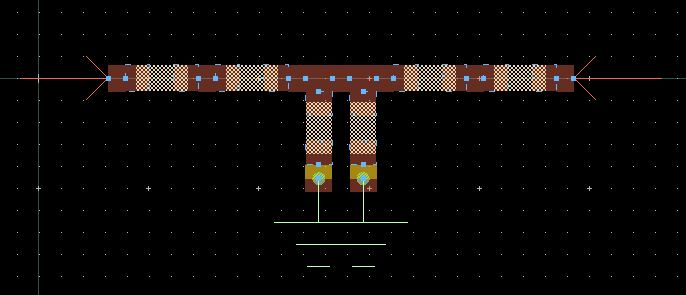
\includegraphics[width=0.5\textwidth]{images/cosimulation_inform/example_circuit_bad.JPG} }%
	    \quad
	    \subfloat[][Filter laid out using knowledge from study]{ 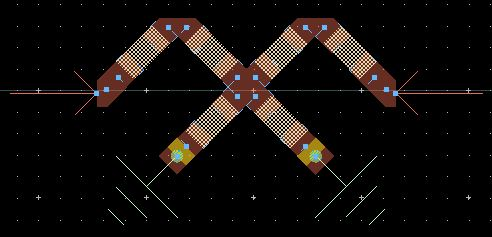
\includegraphics[width=0.4\textwidth]{images/cosimulation_inform/example_circuit_good.JPG}  }
	    \caption{Tee topology Chebyshev band pass filter, without and with using results of study.}
	    \label{fig:better_layout} %
    \end{figure} 
    
    \subsection{Summary}
    In this chapter, the effects of component type, case size, distance and angle are investigated on the responses of s-parameter error and shift in first SRF.
    Statistically significant effects are explored, and and a behavioral model of coupling was developed to inform whether or not the use of full-wave component models is appropriate.
    Also, the efficacy of the brick model in predicting coupling on this fixture is briefly explored, and a design example showing how to apply the principles learned in this chapter is presented.

%%%%%%%%%%%%%%%%%%%%%%%%%%%%%%%%%%%%%%%%%%%%%%%%%%%%%%%%%%%%%%%%%%%%%%%%%%%%%
% % 7-Element Quadrature Coupler
% 	\usfchapter{DESIGN OF 7-ELEMENT QUADRATURE COUPLER}

%       A principal component of many microwave designs is the coupler. As
%     the allotment of physical space for microwave designs decreases,
%     distributed implementations of quadrature couplers become less
%     attractive to the designer. However, for some designs, the use of a
%     monolithic microwave integrated circuit (MMIC) process to provide the best miniaturization is unavailable. This
%     leaves the discrete component lumped-element quadrature coupler as a
%     good solution for designs which are to be produced in small quantity,
%     with relatively quick and inexpensive design iterations. A similar
%     coupler to the one proposed is shown in [dunleavy+ashok white paper],
%     which demonstrates the concept in a microstrip implementation. In the
%     interest of making the smallest design possible, this coupler will be
%     implemented using the Grounded Coplanar Waveguide (GCPW) medium, and
%     using 0402 package size components. The topology of the coupler is
%     shown below:
    
    
%     \begin{center}
%       \begin{circuitikz}
%       \draw
%       (0,0) to [short,o-*] (2,0) to [L,l_=$L$] (7,0) to[short,*-o] (9,0)
%       (2,0) to[C,l_=$C$] (2,3) (7,0) to [C,l_=$C$] (7,3)
%       (2,3) to[L,l_=$L$] (7,3)
%       (2,3) to[C,l_=$C$] (2,6) (7,3) to [C,l_=$C$] (7,6)
%       (0,6) to [short,o-*] (2,6) to [L,l_=$L$] (7,6) to[short,*-o] (9,6)
%       ; 
%       \end{circuitikz}
%     \end{center}
    
%     \subsection{Analysis}
%     \label{sec:org07519ea}
%       As shown in [3], the topology of this coupler can be understood
%     with an even and odd mode analysis, in which the values of inductance
%     and capacitance in the coupler are taken to be
    
%     $$ L = \frac{Z_0}{\omega}, \qquad \qquad C = \frac1{Z_0 \omega} $$
    
%     Given our design frequency of 2.45 GHz, and a system \(Z_0\) of 50
%     \(\Omega\), we find that the necessary L and C needed for our coupler
%     is:
    
%     $$ L = \frac{50}{2\pi\cdot2.45E9} = \boxed{3.248E-9}, \qquad \qquad C
%     = \frac1{50\cdot2\pi\cdot2.45E9} = \boxed{1.299E-12}$$
    
%     \subsection{AWR Simulation}
%     \label{sec:orge682645}
%     \subsubsection{Ideal Circuit}
%     \label{sec:orgb17be8f}
    
    
%     \subsubsection{Parasitic Effects and GCPW Interconnects}
%     \label{sec:orge93be39}
%     \subsection{HFSS Simulation}
%     \label{sec:org6703f31}
%     \subsubsection{Simple Lumped-Element Model}
%     \label{sec:org7a5b536}
%     \subsubsection{Complete Lumped-Element Model}
%     \label{sec:orgafdc66f}
%     \subsection{Measurement}
%     \label{sec:orgeec3857}
%     \subsection{Comparison}
%     \label{sec:org961deaf}
%%%%%%%%%%%%%%%%%%%%%%%%%%%%%%%%%%%%%%%%%%%%%%%%%%%%%%%%%%%%%%%%%%%%%%%%%%%%%
% Reconfiguring of Chip Antenna Layout as Edge-Mount
    \usfchapter{RECONFIGURATION OF CHIP ANTENNA LAYOUT AS EDGE-MOUNT}
    
    \subsection{Full-Wave Lumped Element and Antenna Models in Antenna Design}
    Just as full-wave passives models can model the electromagnetic fields produced by components to give the microwave designer a picture of interaction between components, full-wave antenna models similarly model the impedance and radiated fields of a packaged antenna.
    Full-wave models of packaged antennas allow one to change antenna launches in order to meet other design requirements, and then simulate to make sure that the antenna and launch will still perform as desired. 
    Though models of small, chip antennas which might be used in mobile applications are discussed in this chapter, 3-D modeling of many different types of antennas have proven successful, even without knowing their exact geometries, as is shown in  \cite{antenna_modeling}.
    
    Perhaps the field of antenna design which would benefit most from introduction of full-wave component models is reconfigurable antenna design. 
    Often, PIN diodes or other RF switches are used to electrically connect different segments of such an antenna design. 
    The behaviour of these components is unlikely to match vendor supplied data in the case that these components were characterized with a ground plane which is not present in a prospective design. 
    In \cite{pin_diode_ckt}, the process of developing equivalent circuit models of lumped components is used in this context with good results. 
    The downside of this approach, however, is that it requires the designer to manufacture and measure test fixtures for these components in order to characterize them, and that this approach must be repeated anytime the component is to be used on a new substrate. 
    
    In addition of reconfigurable antennas, many antenna designs also make use of passive lumped elements for the purposes of loading and miniaturization.
    In \cite{pifa_lumped_elements}, a planar inverted-F antenna makes use of a chip inductor and capacitor in order to reduce the total length of the design, and in \cite{mumcuCapacitors} a loop is also miniturized with the use of loading capacitors. 
    
    The most common inclusion of lumped elements in an antenna design by far is their use in a matching network. 
    For this application, equivalent circuit models will do the job correctly most of the time, provided that they are appropriate for the medium and substrate, and that they are spaced out enough to ensure no mutual coupling. 
    However, there are many cases in matching where this is not the case.
    Since the band that the antenna will be matched over will be widest when the matching network is closest to the antenna and the fact that compactness is desired, the designer is incentivized to put the components in non-microstrip mediums, and close together. 

    For example, Figure \ref{fig:5500_matching_network} below shows a Johanson 5500AT07A0900 chip antenna with a matching network which occurs where the feed line loses half of the ground plane right at the edge of the circuit board, whose matching will be investigated in depth in the next section. 
    
    \begin{figure}[H]
		\begin{center}
        	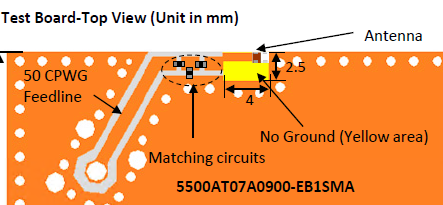
\includegraphics[width=4.5in]{images/2450_reconfig/5500_dev_board.PNG} 
			\caption{Matching network for Johanson 5500AT07A0900 chip antenna with proximity to ground plane discontinuity.} 
			\label{fig:5500_matching_network}
		\end{center}
	\end{figure}    
    
    Over the course of this chapter, an example of the accuracy with which you can represent designs with full-wave models, and an example of how they might be employed to create new designs are presented. 
    
    \subsection{Simulation of an Existing Design in HFSS}

    In order to show the efficacy of the models, the previously mentioned 5500AT07A0900 chip antenna evaluation board was completely modeled in HFSS, and it's simulated and measured input impedance and radiation pattern are presented.
    Besides this section's intended purpose of showing the accuracy of the models employed, a 3-D model of an existing design may still be useful for the purposes of running a yield analysis, or as a starting place for a new design.

    From the datasheet, the design is optimized to be matched to 50 $\Omega$ at 5.5 GHz.
    This is acheived to under -10 dB $S_{11}$ for a bandwidth of about 300 MHz, from around 5.4 GHz to 5.7 GHz.
    The antenna, when mounted on the recommended launch pattern, is relatively omnidirectional, with about 0.5 dBi of gain typical in the plane of the PCB (or ``Azimuth'' as it will be referred to later).
    Figure \ref{fig:5500_real} shows the evaluation board received by Johanson. Note the presence of four objects besides the PCB -- the antenna, two capacitors, and a connector.
    The values of the two capacitors used in the evaluation board are given, as can be seen in Figure \ref{fig:5500_datasheet_vals}.
 
	\begin{figure}%
	    \subfloat[][Side view]{ 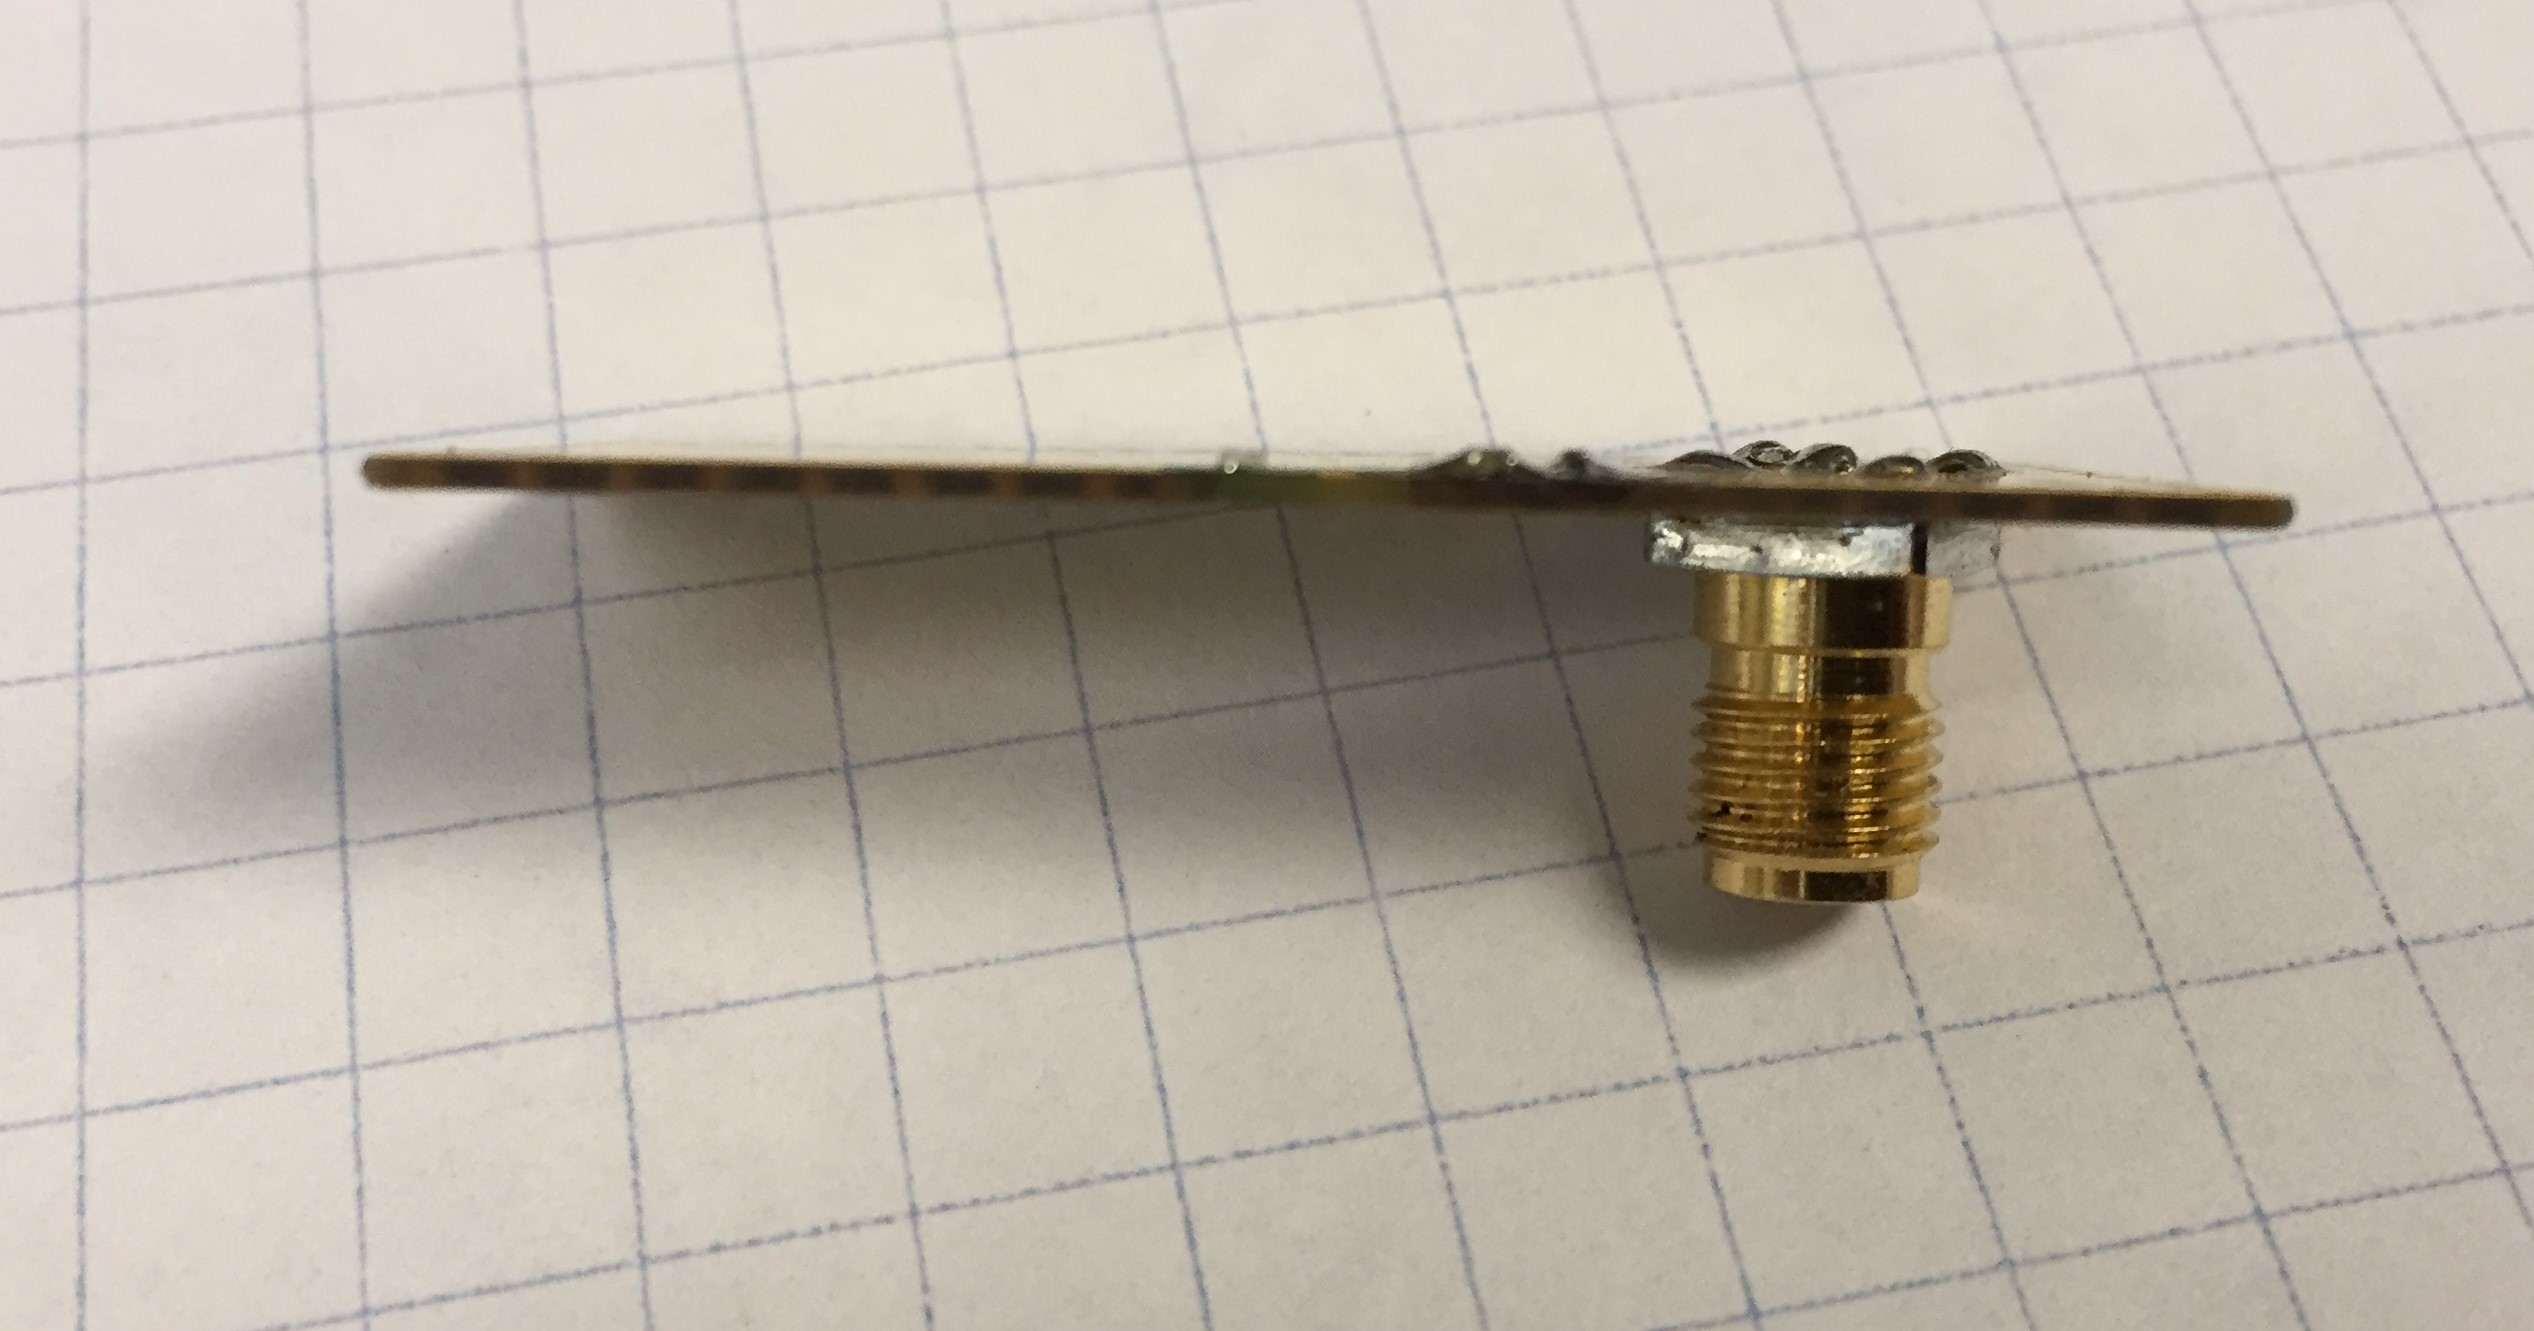
\includegraphics[width=0.5\textwidth]{images/5500_simulation/5500_board_side.JPG}  } %
	    \subfloat[][Top view]{ 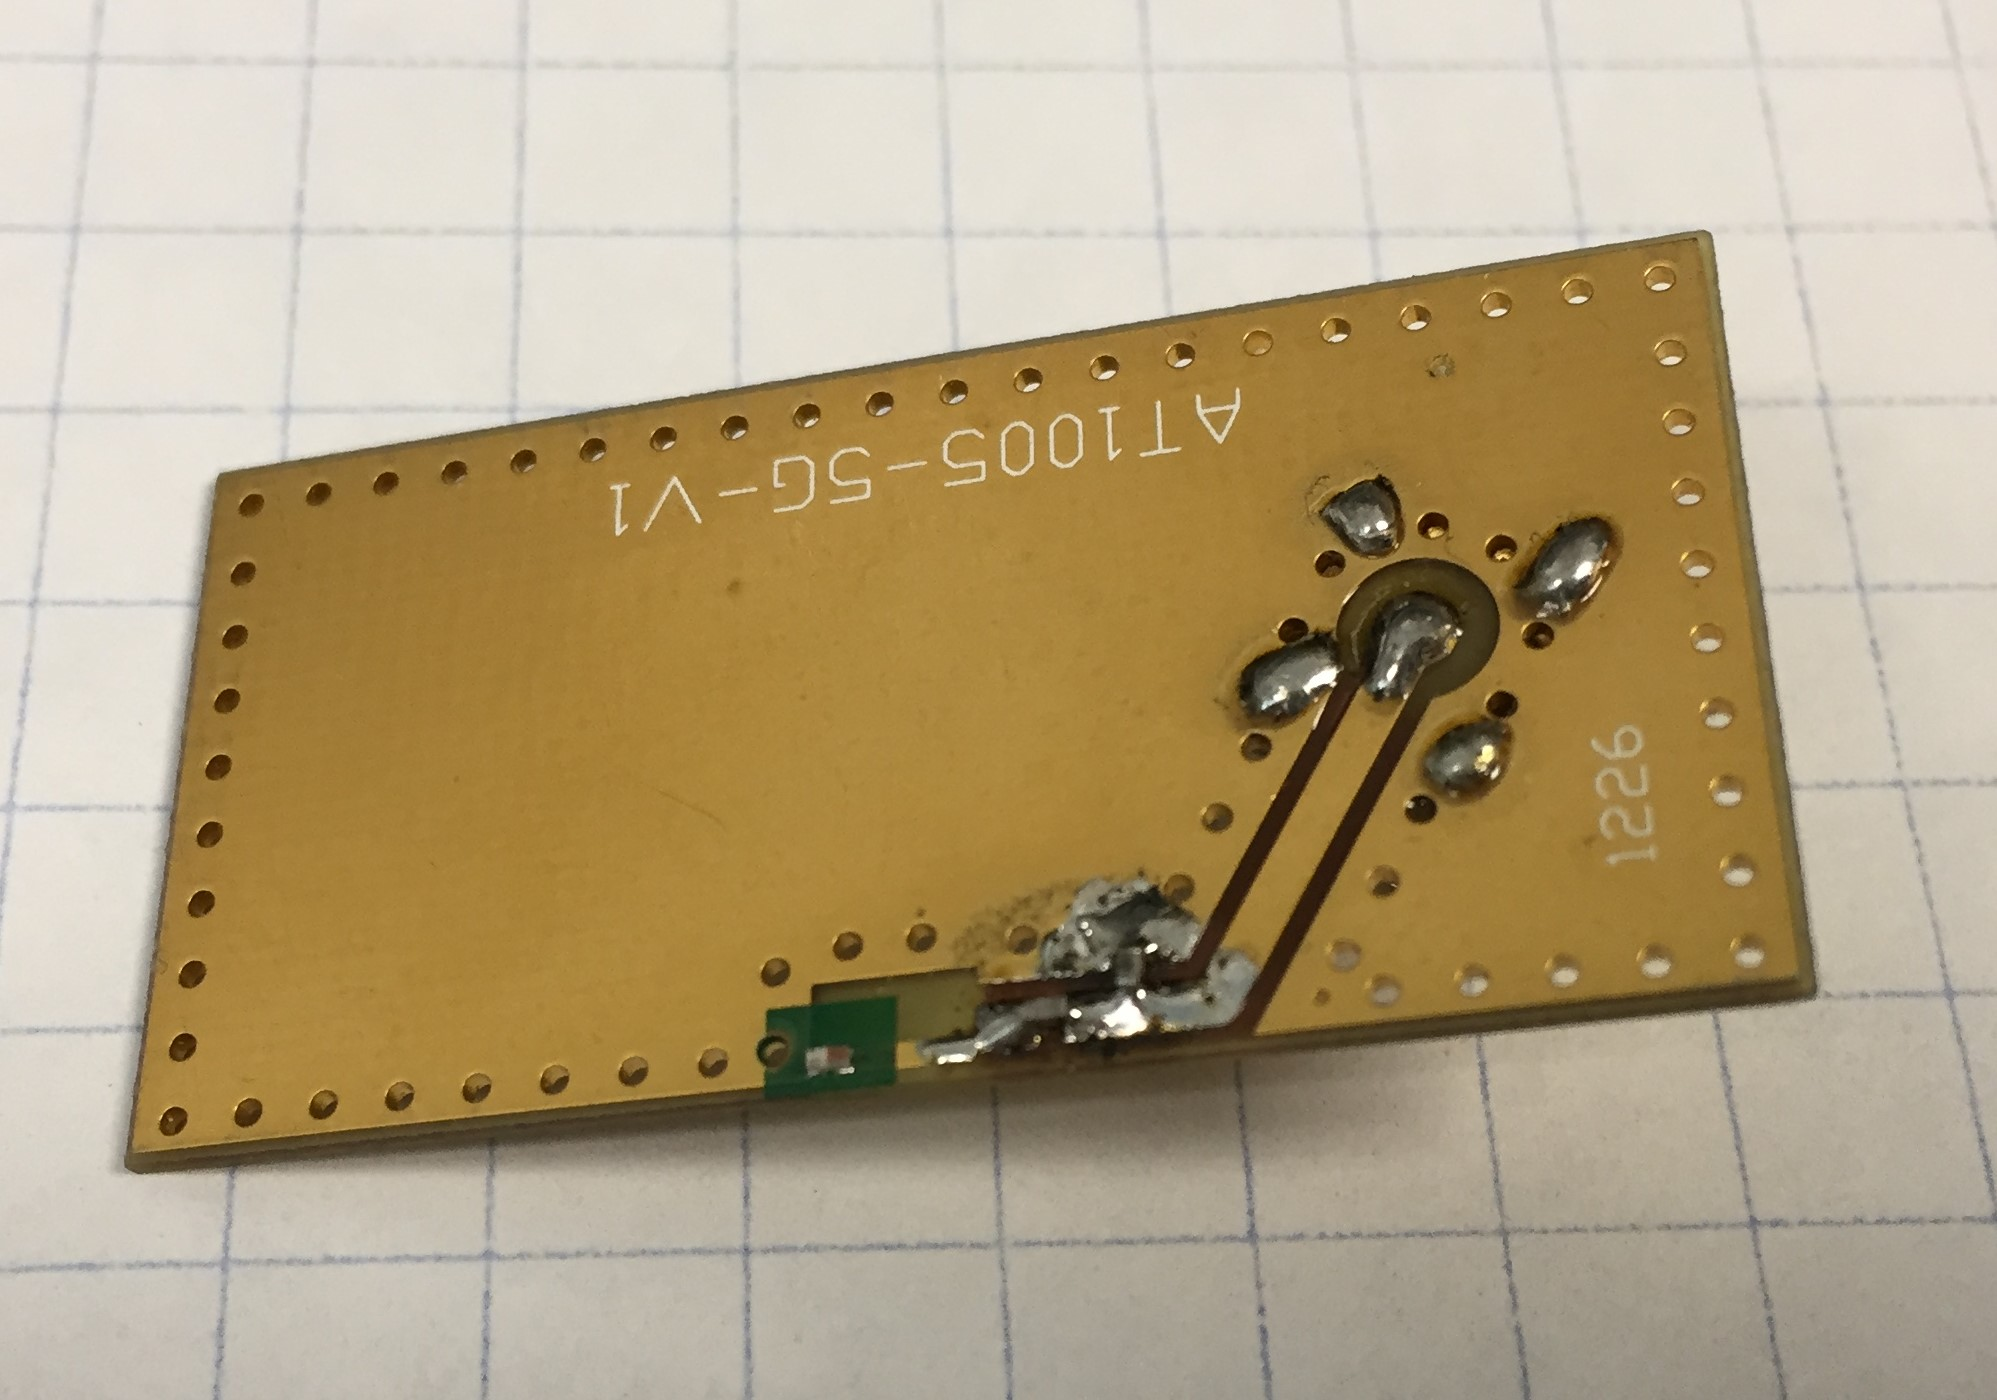
\includegraphics[width=0.47\textwidth]{images/5500_simulation/5500_board_top.JPG}  }
	    \caption{Phyiscal 5500AT07A0900 evaluation board received from Johanson.}%
	    \label{fig:5500_real} %
    \end{figure} 
    
    \begin{figure}[H]
		\begin{center}
        	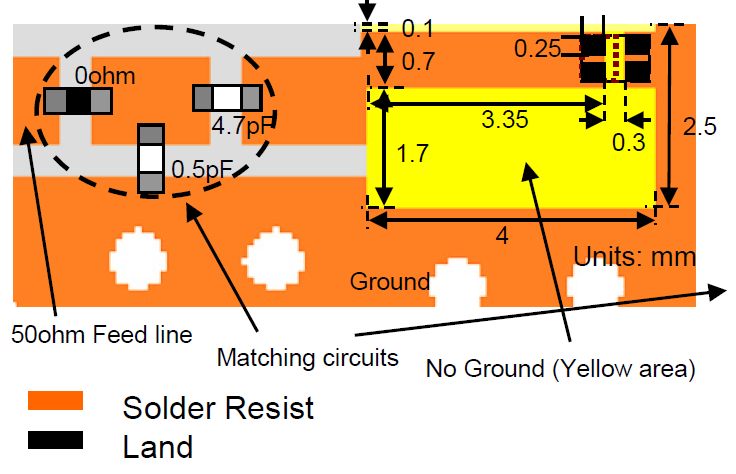
\includegraphics[width=4in]{images/5500_simulation/5500_layout_datasheet.PNG} 
			\caption{Values for two capacitor L section match as shown in datasheet} 
			\label{fig:5500_datasheet_vals}
		\end{center}
	\end{figure}  

    Since the antenna evaluation board is from Johanson, it is not specified in the datasheet, but assumed from the appearance that the 0201 capacitors are the low tolerance R05S capacitors also from Johanson, which is a family whose response is well predicted by it's Modelithics equivalent circuit model together with the brick representation of the package.
    % TODO include the specific name of the connector
    The panel-mount SMA connector is a very common connector, whose full-wave representation was recently constructed and measurement validated by Modelithics.
    Finally, Johanson provided the model of the 5500AT07A0900, as well as geometry for their evaluation board which was read into ANSYS HFSS with a stackup to complete the modeled version of the board. 
    The complete HFSS model of the board and all of it's components can be seen in \ref{fig:5500_hfss_model}.
    Note that the 0 ohm resistor is not present in the simulated design, but rather the gap for the component just removed and filled with copper.
    This was done to ensure consistency with the measured 5500AT07A0900 evaluation board, which simply had a solder bridge across the gap in question as can be seen in Figure \ref{fig:5500_real}.
    Similarly, the signal pin and four grounding/mounting legs were made to be shorter, again to be consistent with the received evaluation boards. 
    The simulation was set up to find S-parameters, as well as the radiation pattern of the antenna. 
    All models were dropped into the simulation as-is, with the exception of the panel mount 3.5 mm SMA connector whose geometry stayed the same, but the de-embed length of the included wave port of which was tuned to match the phase of the measured data.

    \begin{figure}
		\begin{center}
        	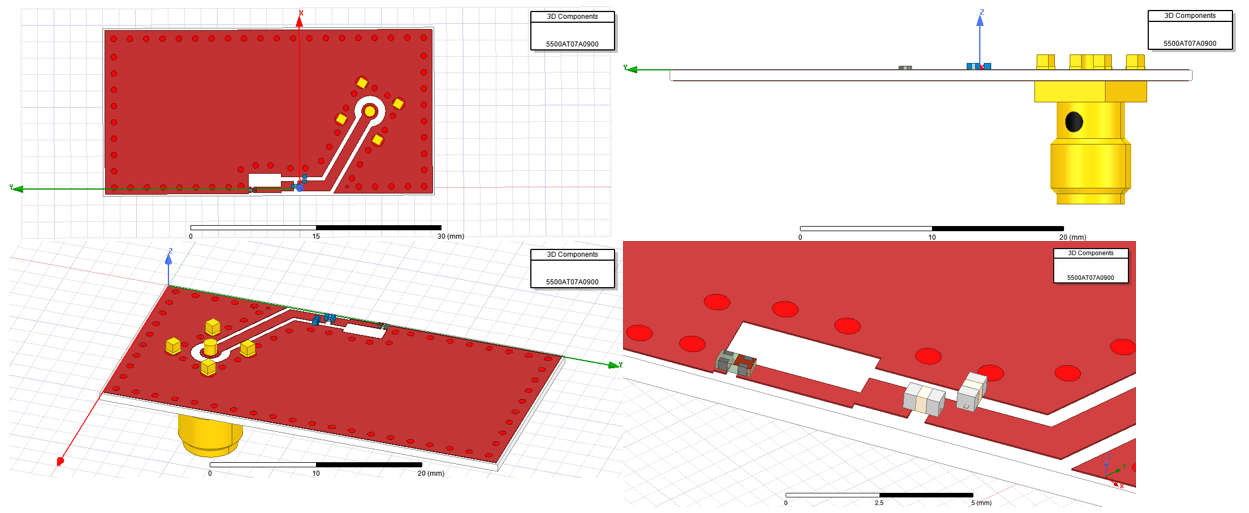
\includegraphics[width=\textwidth]{images/5500_simulation/model.png} 
			\caption{HFSS model of 5500AT07A0900 dev board complete with capacitor models and connector model} 
			\label{fig:5500_hfss_model}
		\end{center}
    \end{figure}    
    
    As can be seen in Figures \ref{fig:5500_smith} and \ref{fig:5500_log_mag}, there is a good agreement between the HFSS simulation with all of the components present and the measurement. 
    The traces which are not the measured data are the simulation in various stages of accuracy; first with reference plane on the board and no brick model, then with reference plane on the board and the brick model, and lastly with brick models and the connector model. 
    The -10 dB return loss bandwidth and series resonant frequencies between the two are almost exactly the same. 
    In \ref{fig:5500_log_mag} it can be seen that the two simulations that had the brick models predicted the resonance of the board correctly, while the only simulation which did not utilize them predicted the resonance to be about 250 MHz higher than it was supposed to be.
    The added accuracy due to the addition of the connector model is more apparent on the Smith chart in \ref{fig:5500_smith}.
    Note how the connector mainly acts like a length of transmission line, having the largest effect on the phase of the input impedance.
    This can also be seen in Figure \ref{fig:5500_smith}, as the response of the simulation with the connector is rotated on the Smith chart to match the phase of the measured data, while the phases of the simulations without the connector do not. 

    % TODO add figures showing cosimulation, brick model cosimulation, and brick model with connector to clarify
    \begin{figure}[H]
		\begin{center}
        	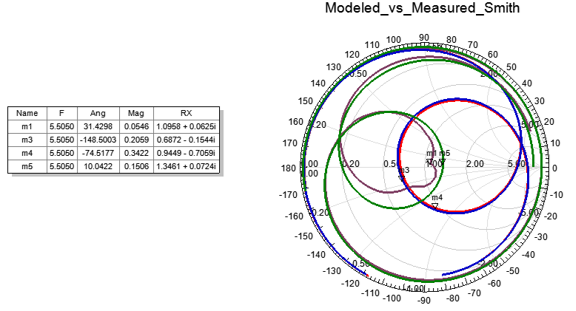
\includegraphics[width=\textwidth]{images/5500_simulation/s11.png} 
            \vspace{-\topsep}
            \begin{itemize}
                \centering
                \setlength{\parskip}{0pt}
                \setlength{\itemsep}{0pt} 
                \color{violet}
                \item Measured
                \color{green}
                \item Simulation with Full-Wave Models and Connector
                \color{blue}
                \item Simulation with Full-Wave Models and No Connector
                \color{red}
                \item Co-simulation with Circuit Models and No Connector
            \end{itemize}
        \vspace*{-9pt}

			\caption{Smith chart representation of 5500 evaluation board input impedance with various simulations v.s. measured data}  % TODO add colors explaining various traces
			\label{fig:5500_smith}
		\end{center}
    \end{figure}    

    \begin{figure}[H]
		\begin{center}
        	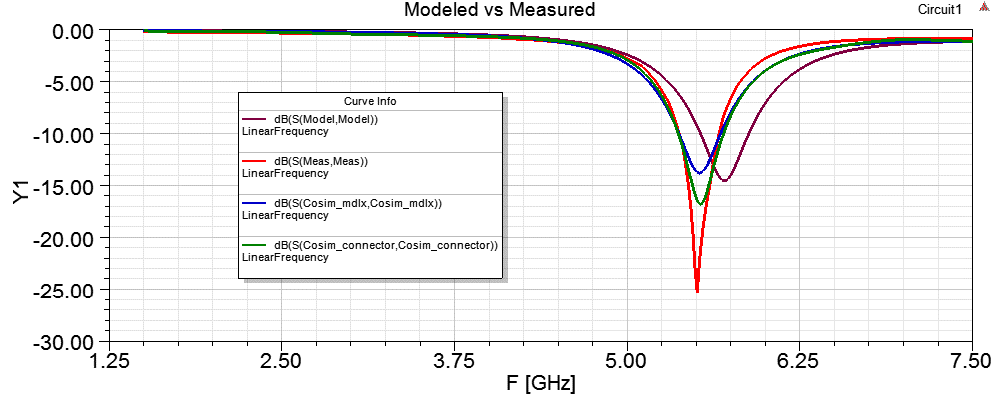
\includegraphics[width=\textwidth]{images/5500_simulation/s11_log_mag.png} 
            \vspace{-\topsep}
            \begin{itemize}
                \centering
                \setlength{\parskip}{0pt}
                \setlength{\itemsep}{0pt} 
                \color{red}
                \item Measured
                \color{green}
                \item Simulation with Full-Wave Models and Connector
                \color{blue}
                \item Simulation with Full-Wave Models and No Connector
                \color{violet}
                \item Co-simulation with Circuit Models and No Connector
            \end{itemize}
            \vspace*{-9pt}
			\caption{Log mag representation of 5500 evaluation board input impedance with various simulations v.s. measured data} 
            \label{fig:5500_log_mag}

		\end{center}
    \end{figure}    

    The realized gain of the antenna was measured using USF's anechoic chamber antenna test station, and is also predicted reasonably well by the simulation.
    The two nulls near 30 and -30 degrees are present in the simulation, but the average realized gain in the azimuth plane is low by about 3.5 dB. 
    % TODO discuss if this is true
    This may have been a problem with the single port approach of the brick model, as non-physical excitations needed to be pushed from the circuit simulation back to the full-wave simulator in order to model the internal impedance of the brick capacitor.
    
    In conclusion, the full-wave models used worked in conjunction to provide an excellent prediction of the input impedance and good prediction of the radiation pattern of the 5500AT07A0900 evaluation board.
    
    \definecolor{darkgreen}{HTML}{277700}

    \begin{figure}[H]
		\begin{center}
        	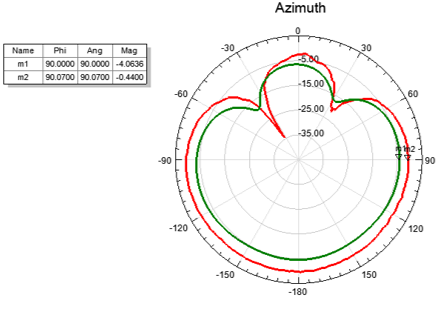
\includegraphics[width=\textwidth]{images/5500_simulation/azimuth.png} 
            \vspace{-\topsep}
            \begin{itemize}
                \centering
                \setlength{\parskip}{0pt}
                \setlength{\itemsep}{0pt} 
                \color{red}
                \item Radiation pattern as measured in anechoic chamber
                \color{darkgreen}
                \item Radiation pattern from simulation with excitations from circuit simulation.
            \end{itemize}
            \vspace*{-9pt}
            
			\caption{Measured v.s. simulated realized gain of 5500 evaluation board} 
			\label{fig:5500_azimuth}
		\end{center}
            
	\end{figure}    


    \subsection{Reconfiguration of Antenna Layout}
    
    The antenna that will be used to demonstrate this design flow is the Johanson 2450A18A100 chip antenna, designed for Wi-Fi and bluetooth applications at 2.45 GHz.
    The original layout of the antenna, pictured in Figure \ref{fig:2450_dev_board}, was realized on 30 mil Rogers 4003C, and had a $S_{11}< -10 $ dB bandwidth of 220 MHz centered around the center frequency. 
    
    
    \begin{figure}[H]
		\begin{center}
        	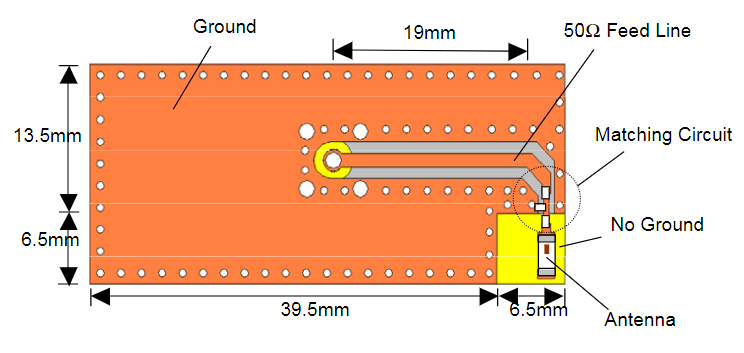
\includegraphics[width=\textwidth]{images/2450_reconfig/2450_dev_board.png} 
			\caption{Evaluation board layout for the Johanson 2450A18A100 chip antenna.} 
			\label{fig:2450_dev_board}
		\end{center}
	\end{figure}    
	
    \begin{figure}[H]
		\begin{center}
        	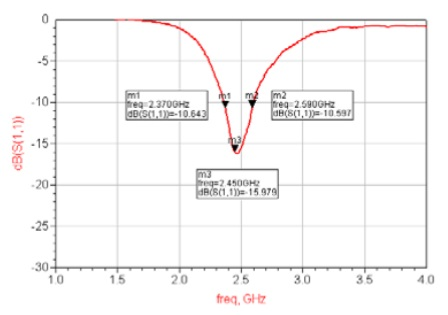
\includegraphics[width=4in]{images/2450_reconfig/datasheet_response.jpg} 
			\caption{Log mag of input impedance as shown in 2450A18A100 datasheet.} 
			\label{fig:datasheet_s11}
		\end{center}
	\end{figure}    
	
	It was decided to revise the original corner-mount layout to be an edge-mount layout --- which both required tuning of the launch using the antenna model, and the synthesis of a new matching network with full-wave component models.
	This revision is certainly something that could be necessary as the result of another design constraint, such as the ability to cascade many of these antenna launches into an array, or the need to make room for PCB fasteners at the edge of a board for better mechanical performance of a hypothetical design.
	Since there is no matching at this point in the design, the Q and realized gain of the layout were the performance metrics optimized against.
	As a network with a higher maximum Q means a lower bandwidth, this metric was optimized to be as small as possible, and the maximum out of any realized gain in the plane perpendicular to the direction of the antenna was also optimized for.
	
	At the very beginning, the line had simply been terminated in the antenna in an area of the PCB with no ground plane underneath.
	This resulted in an antenna impedance with a Q that was several times that of evaluation board when simulated at the same reference plane, which can be seen compared to that of the evaluation board in Figure \ref{fig:2450_first}.
	As shown, the Q incurred when the antenna is simply placed at the edge of the line was about 52, compared to the evaluation board's Q of 13. Having this high of a Q would result in a maximum bandwidth of only 47 MHz from the following relation valid for lossless, linearly polarized, high Q antennas:
	
	$$ BW_{max} = \frac{f}{Q} = \boxed{47 \text{MHz}}, \qquad Q >> 1 $$
	
    Adjusting various dimensions of the cut, how far the antenna protruded into the ground plane cutout, and trying different ways of grounding the rim of the cutout didn't do anything significant to lower the Q of the antenna.
	
	\begin{figure}%
	    \centering
	    \subfloat[][Evaluation Board Model]{ 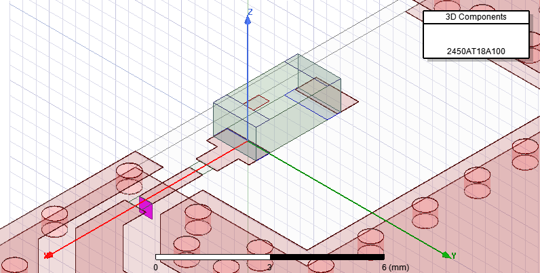
\includegraphics[width=2.5in]{images/2450_reconfig/first_eval_model.png}} %
	    \quad
	    \subfloat[][First Board Model]{ 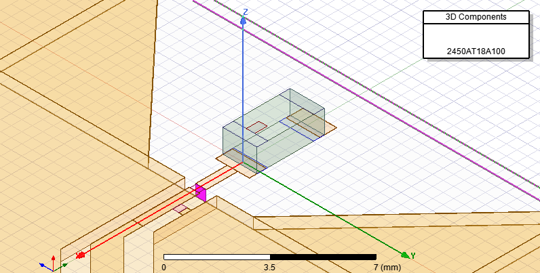
\includegraphics[width=2.5in]{images/2450_reconfig/first_reconfig_model.png}  } %
	    \break
	    \subfloat[][Evaluation Board Q]{ 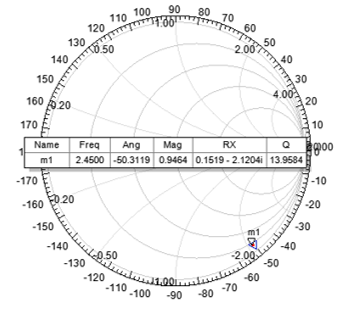
\includegraphics[width=2.5in]{images/2450_reconfig/first_eval_q.png}  } %
	    \quad
	    \subfloat[][First Board Q]{ 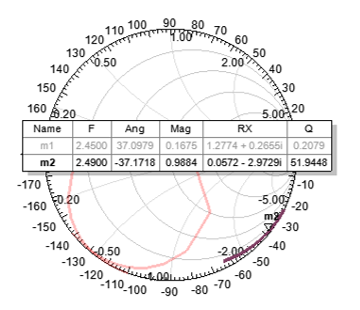
\includegraphics[width=2.5in]{images/2450_reconfig/first_reconfig_q.png}  }
	    \caption{Comparison of HFSS performance of evaluation board and first attempt at reconfiguration.}%
	    \label{fig:2450_first} %
	    \vspace{4in}
    \end{figure} 
	
	
	Eventually, the need for an unbalanced ground plane was realized after discussion with Dr. Mumcu who suggested that the ground plane may be acting as the other arm of a dipole where the first arm is formed by the chip antenna, and the feed leading up to it.
	The first unbalanced configuration of the antenna launch is shown in Figure \ref{fig:starting_point}, in which you can see a view of the HFSS model of the board, as well as the simulated results.
	Adding this asymmetrical ground plane had a dramatic effect on the Q and realized gain of the antenna.
	The Q decreased from 52 shown in Figure \ref{fig:2450_first}, down to 16.9 shown in Figure \ref{fig:starting_point}, and likewise the gain increased from -15 dBi typical up to -10 dBi typical. 
	
	\begin{figure}%
	    \centering
	    \subfloat[][3-D Model]{ 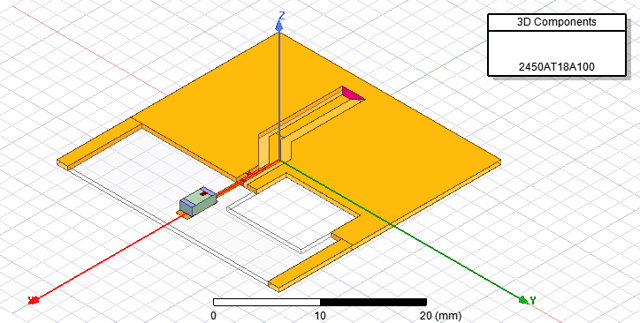
\includegraphics[width=4in]{images/2450_reconfig/starting_point.png}} %
	    \break
	    \subfloat[][Impedance @ 2.45 GHz (reference plane at end of GCPW line)]{ 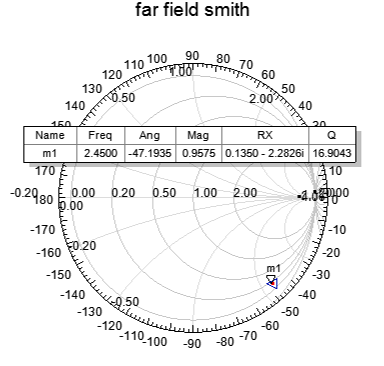
\includegraphics[width=2.5in]{images/2450_reconfig/starting_point_q.png}  } %
	    \qquad
	    \subfloat[][ZY cut of realized gain pattern]{ 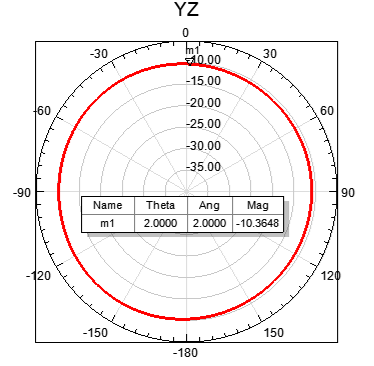
\includegraphics[width=2.5in]{images/2450_reconfig/starting_point_radn.png}  }
	    \caption{HFSS model and simulated results of starting reconfig board.}%
	    \label{fig:starting_point} %
	    \vspace{3.5in}
	    
    \end{figure} 
    
	Q and realized gain of the design was most sensitive to the how far the newly introduced cut extended into the ground plane. 
	After tuning of this parameter, the length that the antenna extends out past where the ground plane ends, the width of the cut, and a few others, the Q and gain of the design got even better.
	The final model of the board as well as its performance can be seen in Figure \ref{fig:finish_point} -- where the Q of the design in 6.88, and the maximum realized gain in YZ plane is -5.3 dBi. 

	\begin{figure}%
	    \centering
	    \subfloat[][3-D Model]{ \includegraphics[width=4in]{images/2450_reconfig/finish_point.png}} %
	    \break
	    \subfloat[][Impedance @ 2.45 GHz (reference plane at end of GCPW line)]{ \includegraphics[width=2.5in]{images/2450_reconfig/finish_point_q.png}  } %
	    \qquad
	    \subfloat[][ZY cut of realized gain pattern]{ \includegraphics[width=2.5in]{images/2450_reconfig/finish_point_radn.png}  }
	    \caption{HFSS model and simulated results of reconfig board after tuning.}%
	    \label{fig:finish_point} 
	    \vspace{4in}
    \end{figure} 

    
    \subsubsection{Matching with Circuit Models}
    
    Now that a viable antenna layout had been found, the next step was to match the circuit through the use of co-simulation and circuit models.
    Figure \ref{fig:2450_mdlx_ckt_cosim} shows how the cosimulation was set up -- in the full-wave simulator, one can see the differential ports where the impedance of the capacitors are to be attached across. 
    This design uses the same single port approach as explained in section \ref{differential_port_explanation}, but note carefully that no brick model is used here. 
    The point that was to be matched to 50 $\Omega$ was in the bottom right hand side of the Smith chart, as is demonstrated by the marker on the trace in Figure \ref{fig:finish_point} (b). 
    Resulting from this fact, a two inductor shunt-series L-section match could have been used, but 3 inductors were chosen in a tee topology instead as to allow finer control over the specific impedance matched to.
    The values of the inductors seen in the circuit co-simulation in Figure \ref{fig:2450_mdlx_ckt_cosim} were tuned by hand to obtain a match which had similar bandwidth to that of the matching network on the original design shown in \ref{fig:datasheet_s11}. 
    By this method, the inductor values shown in Table \ref{tbl:2450_ckt_vals} below were obtained:
        
	\floatstyle{plaintop}
	\restylefloat{table}					
	\begin{table}[H]
	\centering
	\begin{tabular}{|c|c|}
		\hline  
		 Parasitic Name & Value \\
		 \hline
		 $L_{series2}$ & 3.3 nH \\
		 \hline
		 $L_{shunt}$ & 4.7 nH \\
		 \hline
		 $L_{series2}$ & 2.7 nH \\
		 \hline
	\end{tabular}
	\caption{Values of components in 2450A18A100 reconfiguration board matching network which gave the best best circuit co-simulation match.}
	\label{tbl:2450_ckt_vals}
	\end{table}

    This combination of component values, which were obtained with a relatively quick full-wave simulation of the antenna board and circuit tuning, constitute the results of the completed first step of the design process outlined in Section \ref{cosimulation_inform_3D}.

    \begin{figure}[H]
		\begin{center}
        	\includegraphics[width=0.7\textwidth]{images/2450_reconfig/mdlx_circuit_cosim.PNG} 
			\caption{Matching of reconfig board using Modelithics circuit models} 
			\label{fig:2450_mdlx_ckt_cosim}
		\end{center}
	\end{figure}    
	
    \subsubsection{Matching with 3-D Model}
    
    Next in the process of 3-D matching is the full-wave gradient descent. 
    As explained in section \ref{cosimulation_inform_3D}, since full-wave optimization with component models is relatively time intensive when compared to circuit co-simulation, using co-simulation to first approach the correct values is very important to getting a result quickly.
    Figure \ref{fig:full_wave_match_circuit_vals} shows the full-wave simulation representation of the inductors with the values found in the previous section.
    Since these models represent the interaction that would actually occur between the components, the input impedance of this simulation was of course different than the one found by the co-simulation. 
    Though the resonance stayed at about 2.45 GHz, the return loss at this frequency decreased to -4.6 dB, which can be seen as the blue trace in Figure \ref{fig:2450_grad_descent}. 
    
    \begin{figure}[H]
		\begin{center}
        	\includegraphics[width=\textwidth]{images/2450_reconfig/full_wave_match_circuit_vals.PNG} 
			\caption{Full-Wave representation of matching network with best circuit co-simulation values marked in nanohenries.} 
			\label{fig:full_wave_match_circuit_vals}
		\end{center}
	\end{figure}    
	
	Design using the full-wave component models was started at the values given in Table \ref{tbl:2450_ckt_vals}, which is shown as the point in Figure \ref{fig:2450_grad_descent}. 
	A few words remind the reader of what exactly the gradient descent 3-D plot in Figure \ref{fig:2450_grad_descent} represents. 
	Each index is labeled with a number, which is the index of a specific component value in the MLG0603S family, with 0 being the index of the first component value, and increasing with each subsequent 3-D model value. 
	So, a point in this space corresponds to a specific permutation of 3 component models, one for each place in the matching network. 
	Each one of these points has also an input impedance response against frequency associated with it which can be obtained by running the full-wave simulation with that collection of part values in that order.
	From this response, a metric can be calculated to quantify how well matched the network with these values is at the design frequency, as is illustrated in Figure \ref{fig:grad_desc_cost_calc}.
	For this particular simulation, the cost bandwidth was defined to be 200 MHz from one side of the cost kernel's nonzero portion to the other side, which means that the simulator only had to simulate from 2.35 to 2.55 GHz in order to calculate the cost.
    This cost is represented in the 3-D plot in Figure \ref{fig:2450_grad_descent} as the color of each 3-D point, with a warmer color for a lower cost (more desirable), and cooler color for a higher (less desirable).
    In the visualization in question, the 3 separate gradient descents which were run from different starting points in the solution space are shown. 
	
    \begin{figure}[H]
		\begin{center}
        	\includegraphics[width=\textwidth]{images/2450_reconfig/gradient_descent.PNG} 
			\caption{Plot showing improvement of matching network cost v.s. values combination, and corresponding response on Smith chart} 
			\label{fig:2450_grad_descent}
		\end{center}
	\end{figure}    
    
    In addition to visualizing the solution space for this design, this figure handily illustrates a limitation of the gradient descent which designers should always keep in mind when using it, or any local minimum search algorithm.
    Each time one of the groups shown in Figure \ref{fig:2450_grad_descent} terminated, it found a local minimum, which is not necessarily the same thing as the best solution in the solution space.
    Note that the combination of values which the algorithm converged to first (the point directly below the topmost point in the middle cluster) was only halfway to the best cost achieved in this region starting from the best circuit values.
    
    The cluster on the left of the visualization which contained the best 3-D value was started by observing how the impedance of the co-simulated board changed when the inductor values were held constant and simulated in the full-wave simulator.
    As can be seen in the Smith chart in Figure \ref{fig:2450_grad_descent}, the impedance of the co-simulation, whose impedance at 2.45 GHz was at 50 $\Omega$, got translated by an impedance of about +100$j$ to the point shown by the marker on the blue trace. 
    With the the thinking that this change would be relatively consistent, the circuit co-simulation was matched to the impedance 50-100j $\Omega$, and this combination of inductor values (seen in the visualization as the point directly above the bottom-most point in the leftmost cluster) was the starting point for the gradient descent which produced the lowest cost combination of inductor values for the full-wave simulation.
    
    The lowest cost combination of values is shown in Table \ref{tbl:2450_3D_vals}, which are considerably different from the best circuit values.
    This should not be taken as evidence that how the cost depends on component values varies too greatly between the full-wave circuit representation of these matching networks, as there are likely many combinations of the two series inductors which give a good match.
    The impedance of this network as it varies with frequency can be seen as the red trace on the Smith chart in \ref{fig:2450_grad_descent}.
	
	\floatstyle{plaintop}
	\restylefloat{table}					
	\begin{table}[H]
	\centering
	\begin{tabular}{|c|c|}
		\hline  
		 Parasitic Name & Value \\
		 \hline
		 $L_{series2}$ & 5.1 nH \\ % TODO figure out what these were
		 \hline
		 $L_{shunt}$ & 3.0 nH \\
		 \hline
		 $L_{series2}$ & 5.1 nH \\
		 \hline
	\end{tabular}
	\caption{Values of components converged to by full-wave gradient descent for 2450A18A100 reconfiguration board matching network.}
	\label{tbl:2450_3D_vals}
	\end{table}
	
    \subsubsection{Measurement}
    
    \indent Finally, the simulated PCB was manufactured, and the components and connector populated.
    A picture of the manufactured and populated antenna board is shown in Figure \ref{fig:irl_antenna_board} (a).
    
    
	\begin{figure}%
	    \subfloat[][Manufactured antenna board with inductor values given in Table \ref{tbl:2450_3D_vals} ]{ \includegraphics[width=0.47\textwidth]{images/2450_reconfig/made_antenna.JPG}  } %
	    \hspace{0.03\textwidth}
	    \subfloat[][Coax to PCB to coax thru structure used to put reference plane of measurement onto board]{ \includegraphics[width=0.47\textwidth]{images/2450_reconfig/thru.JPG}  }
	    \caption{2.45 GHz antenna reconfiguration board and thru test structure for de-embedding}%
	    \label{fig:irl_antenna_board} %
    \end{figure} 
	
    Like the 5.5 GHz Johanson evaluation board found in the previous section of this chapter, this board was fed using a PCB mount SMA jack.
    Though the reference plane of the simulation is on the PCB itself, the reference plane for the raw measurement was in the middle of the connector, as the measurement was taken using a SMA female Short Open Load Thru (SOLT) calibration. 
    From this measurement,the reference plane was moved up to the same reference plane as the simulation by de-embedding half of a coax to PCB to coax thru structure, pictured in Figure \ref{fig:irl_antenna_board}(b).
    The thru structure used to measure this board was also measured using the coaxial calibration, then half of it's response was found through the use of a technique to split such two-port structures as outlined in \cite{thru_split}.
    
    
    \begin{figure}[H]
		\begin{center}
        	\includegraphics[width=\textwidth]{images/2450_reconfig/final_results.PNG} 
			\caption{Comparison of log magnitude of input impedance for measured, 3-D modeled and circuit modeled boards} 
			\label{fig:2450_final_results}
		\end{center}
	\end{figure}    

    \subsection{Summary}
    In this chapter, antenna designs are modeled which demonstrate the accuracy and convenience of full-wave component models.
    First, a complete 3-D representation of the Johanson 5500 evaluation board is constructed whose simulated input impedance predicts that of the measure data very well over the entire range of the response.
    In addition to this, the radiation pattern of the boards is found to predict the shape measured pattern in azimuth. 
    Finally, the evaluation board for the 2450 was reconfigured to be edge mount to serve as an example of the process by which new designs can be synthesized using full-wave models. 
    Through this process, -14 dB of return loss is achieved with about 120 MHz of bandwidth in the measured design on the first pass.

    \usfchapter{CONCLUSIONS AND RECOMMENDATIONS}

    In this thesis, the motivation, tools and advice for design using full-wave 3-D component models are described in some detail.  To demonstrate the proposed design methodology, two design examples are presented along with a statistics-based inquiry into inter-component coupling.  The application of these methods to apply to designs using both lumped and distributed components is becoming more feasible given the advent of 3-D model encryption by commercial companies, that promised to lead to a much wider availability of 3-D models to the design community. 
    It is demonstrated that predictions of antenna design responses which model the change in resonant frequency to within a close approximation can be made, even for situations where lumped components may be mounted closely together and on non-standard interconnect media. 
    The following procedure is recommended to those who wish to have an accurate simulation of the response of passive elements in a configuration other than on microstrip, or in close proximity to one another:

    \subsection{Unusual Configurations}

    If the lumped elements are to be used in an unusual configuration (Antenna loading with no ground plane beneath, 3D printed applications, in between layers of substrate stack up), it is recommended that users first perform a co-simulation with accurate circuit models of the components in question.
    This ensures that the full-wave models have a good starting point in the combination of lumped element values found as optimal by the co-simulation.
    If none are available, ideal circuit representations will suffice to move the combination of values closer to the combination of values that will perform best in the full-wave simulation.
    Since even the highest quality circuit models have parasitics built into them, the designer should not spend an inordinate amount of time optimizing the circuit simulation, but rather move on to full-wave component representations as soon as an acceptable response is achieved. 
    From here, the gradient descent presented or a similar optimization should be conducted until the desired response is achieved.

    \subsection{Close Proximity}

    \indent The next question to address is that of proximity, or: ``For what spacing and orientation do inter-component couplings become significant?''. 
    First, it is recommended that the designer define an acceptable shift in SRF, then consult the coupling behavioral model given in section 2.4.1 if the prospective design has a similar ratio of substrate height to $\epsilon_r$, (0.14 mm for Rogers 4530B).
    If the predicted design frequency shift is within an acceptable range, the designer can proceed to use the circuit co-simulation approach.
    If outside acceptable boundary, the designer should find optimum combination of component values which give the best response in a circuit simulation or co-simulation, then move on to a full-wave optimization. 
        
    \subsection{Opportunities for Further Study}

    \indent Though the implications of accurate full-wave component models have on circuit design is explored in the context of matching networks in this thesis, perhaps a more dramatic effect could be observed by comparing the response of  co-simulated circuit models to full-wave models in the context of antenna loading.
    The conditions in the two matching networks shown were certainly quite different than microstrip (``half grounded co-planar waveguide'' in the case of 5.5 GHz evaluation board design), but the models would be utilized to their fullest potential in antenna loading, as only they can model the effect packages and stored fields have on the antenna's radiation as well.  
    A simple antenna loading application would be a microstrip monopole loaded with an inductor to decrease it's size, or the loop antenna design given in \cite{mumcuCapacitors}. 
    Another good application of brick modeling could be PIN diodes as they are used in a reconfigurable antenna design. 
    The work done in \cite{brick_diode} is similar to this idea, but requires a RC equivalent of the diode to be extracted for each bias it is to be used at.
    This would preclude the need to develop circuit models unique to one stackup, as is done in \cite{pin_diode_ckt}.
    In addition to these applications, as 3-D printed antenna designs gain popularity, a versatile circuit model which would accurately model the response of a component in any configuration will surely become more helpful to the designer.
    This could give the designer the ability to put a matching network closer to the antenna and obtain a better bandwidth performance as a result, using for instance conductive ink deposited to form a CPW medium in which these components could be used. 
    
    With a better picture of component interaction, microwave designers will be able to quickly design smaller and more versatile passive networks.

%%%%%%%%%% Bibliography %%%%%%%%%%%%% 

\usfpagebreak
\addcontentsline{toc}{section}{REFERENCES}
% \renewcommand\bibname{\centering REFERENCES}
\bibliography{thesis}
\bibliographystyle{plain}

%%%%%%%%%% Copyright Permissions %%%%%%%%%%%%% 

\usfpagebreak
\begin{center}
\section*{\centering APPENDIX: COPYRIGHT PERMISSIONS}
\addcontentsline{toc}{section}{APPENDIX: COPYRIGHT PERMISSIONS}
Figures \ref{fig:mdlx3d_comps_paper_fig_7}, and \ref{fig:mdlx3d_comps_paper_fig_7} of \cite{mdlx_3d_models} were used with permission from the copyright holder.
\includegraphics[width=0.85\textwidth]{ieee_copyright_permissions.PNG}
\end{center}


\end{document}